\documentclass[10pt]{usetex-v1}
%\documentclass[10pt,workingdraft]{usetex-v1}

\usepackage[table]{xcolor}% http://ctan.org/pkg/xcolor
\usepackage{epsfig}
\usepackage{url}
\usepackage{times}
%\usepackage{subfigure}
\usepackage{tabularx}
%\usepackage{scalefnt}
%\usepackage{endnotes}
%\usepackage{footnote}
%\usepackage{multirow}
%\usepackage{amsmath}
%\usepackage{amssymb}
%\usepackage{booktabs}
%\usepackage{listings}
\usepackage{vmargin}
\usepackage{cite}
\usepackage{alltt}
%\usepackage{psfrag}
%\usepackage{boxedminipage}
\usepackage{colortbl}
\usepackage{xspace}
%\usepackage[showframe=true]{geometry}
\usepackage{enumitem}
%\usepackage{program}
\usepackage{listings}

%\numberwithin{equation}{section}
% space b/t list \item's
\newcommand{\smallitemsep}      {\setlength{\itemsep}{-0.5ex}}
%\newcommand{\smallitemsep}     {}

\newcommand{\stt}[1]            {\texttt{\small #1}}

% space b/t captions and their floats
\newcommand{\captionsep}        {\vspace{-1.00em}}
\newcommand{\tabcaptionsep}     {\vspace{-0.50em}}
%\newcommand{\captionsep}       {}
% size of caption font
%\newcommand{\captionfont}      \tiny
\newcommand{\captionfont}       \itshape
\newcommand{\capfont}           \small
%\newcommand{\capfont}          {}

\newcommand{\etal}{\emph{et al.}}

% make tables narrower in width so they fit better in twocolumn formats
\addtolength{\tabcolsep}{-0.5\tabcolsep}
% less space between rows of tables
\renewcommand{\arraystretch}{0.95}
%% space between columns in twocolumn mode
%\addtolength{\columnsep}{-0.1\columnsep}

\newenvironment{consistifyoff}[0]{}      {}

\newenvironment{ezbox}[1]%
{
 \footnotesize
 \begin{center}
 \begin{boxedminipage}[t]{#1}
 \begin{alltt}
}
{
 \end{alltt}
 \end{boxedminipage}
 \end{center}
}

\newenvironment{smalltt}%
{
\vspace{-0.5em}
\footnotesize
\begin{alltt}
}
{
\end{alltt}
\vspace{-0.5em}
}

%\lstset{language=C, basicstyle=\ttfamily\small}
\hyphenation{vnode}

% redefine \url font to normal font
\def\UrlFont{\sl\footnotesize}

\begin{document}

\title{Study of Energy Efficiency in BFS Algorithms}

\author{
    \authname{Bharat Singh and Srikant Aggarwal}
    \authaddr{Stony Brook University}
}

\setpapersize{USletter}
% % \setmarginsrb{leftmargin}{topmargin}{rightmargin}{bottommargin}%
% %    {headheight}{headsep}{footheight}{footskip}
\setmarginsrb{25mm}{25mm}{25mm}{15mm}{0mm}{0mm}{10mm}{10mm}

\pagestyle{plain}

%\newcommand{\stt}[1]                    {\texttt{\small #1}}
%\def\gtilda{\kern -.15em\lower .7ex\hbox{\~{}}\kern .04em}

%%%%%%%%%%%%%%%%%%%%%%%%%%%%%%%%%%%%%%%%%%%%%%%%%%%%%%%%%%%%%%%%%%%%%%%%%%%%%%
%%% SQUEEZE SOME SPACES
%\addtolength{\parskip}{4.5\parskip}
%\setlength{\partopsep}{0mm}
%\setlength{\topsep}{0mm}
%\addtolength{\baselineskip}{-0.03\baselineskip}
%\setlength{\parskip}{-0.5ex}
%\renewcommand{\baselinestretch}{0.9}
%\addtolength{\tabcolsep}{-0.5\tabcolsep}
%\setlength{\topsep}{-2.0ex}
%
%% make tables narrower in width so they fit better in twocolumn formats
%\addtolength{\tabcolsep}{-0.4\tabcolsep}
%% less space between rows of tables
%\renewcommand{\arraystretch}{0.95}
%% allow up to 4 floats at top of page (default=2)
\setcounter{topnumber}{4}
\setcounter{dbltopnumber}{8}	% for double-floats
%% allow up to 2 floats at bottom of page (default=1)
\setcounter{bottomnumber}{2}
%% allow up to 8 floats total per page (default=3)
\setcounter{totalnumber}{8}

% %% less space above/below floats that are at top/bottom of pages
\addtolength{\floatsep}{-0.5\floatsep}
\addtolength{\dblfloatsep}{-0.5\dblfloatsep}
% %% less space above/below "h" floats that are in the middle of text
\addtolength{\intextsep}{-0.5\intextsep}
\addtolength{\textfloatsep}{-0.5\textfloatsep}
\addtolength{\dbltextfloatsep}{-0.5\dbltextfloatsep}
% smaller space around captions
\addtolength{\abovecaptionskip}{-0.75\abovecaptionskip}

%% Control floats
\renewcommand{\topfraction}{1.0} % max percentage a float can take at top
\renewcommand{\bottomfraction}{1.0} % max percentage float can take at bottom
\renewcommand{\textfraction}{0.01} % min percentage text can take on page
%\renewcommand{\textfraction}{0.5} % min percentage text can take on page
\renewcommand{\floatpagefraction}{0.99} % min fraction of float page used
\renewcommand{\dblfloatpagefraction}{0.99} % min fraction of float page used

%% space between columns in twocolumn mode
%\addtolength{\columnsep}{-0.1\columnsep}
%% width of text on a page
%\addtolength{\textwidth}{0.01\textwidth}

%%%%%%%%%%%%%%%%%%%%%%%%%%%%%%%%%%%%%%%%%%%%%%%%%%%%%%%%%%%%%%%%%%%%%%%%%%%%%%

%\tableofcontents
\maketitle

\begin{abstract}

% dummy entry to force emacs not to indent abstract text
\vspace{0mm}

%"sales pitch".  a short 1-2 pgfs, few sentences,
%to convince the reader to read the rest.
%
%1. there's a problem
%
%2. what others have done about it (WHY no good)
%
%3. what you did (WHY it's better)
%
%4. WHY your stuff is better (some results?)
%
%No citations.


%Breadth-First Search is an algorithm for traversing or searching tree
%or graph data structures. 
In this paper, we explored existing research
in area of parallel Breadth First Search and benchmarked them in terms
of energy efficiency and related parameters like Memory and Cache
Performance. We also analysed the benchmarking results.

\textbf{Keywords: }CILK, NUMA

\end{abstract}

%%%%%%%%%%%%%%%%%%%%%%%%%%%%%%%%%%%%%%%%%%%%%%%%%%%%%%%%%%%%%%%%%%%%%%%%%%%%%%
%% For Emacs:
% Local variables:
% fill-column: 70
% End:
%%%%%%%%%%%%%%%%%%%%%%%%%%%%%%%%%%%%%%%%%%%%%%%%%%%%%%%%%%%%%%%%%%%%%%%%%%%%%%
%% For Vim:
% vim:textwidth=70
%%%%%%%%%%%%%%%%%%%%%%%%%%%%%%%%%%%%%%%%%%%%%%%%%%%%%%%%%%%%%%%%%%%%%%%%%%%%%%
% LocalWords: eCryptfs, POSIX, UID

\section{Introduction}
\label{intro}

Breadth-first search (BFS) is being used in basically anything that
optimizes for minimum distance in some way.  It is an important kernel
used by many graph-processing applications including GPS based
navigation systems, Social network analysis tools etc.\newline
%islso known as BFS, finds shortest paths from a given source node to
%all other nodes, in terms of the number of edges in the path. It
%starts at the source node and explores the neighbour nodes first
%before moving to the next level neighbours. The traversal technique
%it is being used in basically anything that optimizes for minimum
%distance in some way.  It is an important kernel used by many
%graph-processing applications including GPS based navigation systems,
%Social network analysis tools etc.\newline
In recent years hardware and storage have become cheaper. So to scale
up we deploy multi-cores and heterogeneous computing units on a large
scale. This though speeds up the execution, leads to an increase in
power consumption and hence the maintenance costs. Hence, now a days
energy efficiency of an algorithm is becoming a matter of primary
concern.
\newline
Due to BFS traversal being so commonly used and given
the vast size of graph data sets, it alone accounts for significant
time and energy consumption these days.  This motivated us to explore
energy efficiency of existing BFS traversal techniques, analyse
results and come out with programming techniques which makes it more
energy efficient.
\newline
%Some of the key factors impacting performance are locality, cache
%efficiency, energy and power.  Graph algorithms are becoming
%increasingly important, with applications covering a wide range of
%scales. Computers run graph algorithms that reason about vast amounts
%of data, with applications including analytics and recommendation
%systems. On mobile clients, graph algorithms are important components
%of recognition and machine learning applications.  Typical length:
%1-1.5 pages.
%one-page summary of entire paper: - same 4 steps as abstract, but 1
%pgf each, instead of 1 sentence.  - intro very important: most
%reviewers make up their mind early on.
%When to write intro: - last: to ensure it properly summarizes entire
%paper.  - first: useful as an outline for rest of work
%Often best to write an outline of whole paper/ideas.
The rest of this document is organized as follows.  Section 2
describes background on parallel BFS.  Section 3 describes our
benchmarking setup.  Section 4 describes evaluation plan and results.
Section 5 describes conclusion and future work.

%%%%%%%%%%%%%%%%%%%%%%%%%%%%%%%%%%%%%%%%%%%%%%%%%%%%%%%%%%%%%%%%%%%%%
%% For Emacs:
% Local variables:
% fill-column: 70
% End:
%%%%%%%%%%%%%%%%%%%%%%%%%%%%%%%%%%%%%%%%%%%%%%%%%%%%%%%%%%%%%%%%%%%%%
%% For Vim:
% vim:textwidth=70
%%%%%%%%%%%%%%%%%%%%%%%%%%%%%%%%%%%%%%%%%%%%%%%%%%%%%%%%%%%%%%%%%%%%%%
% LocalWords:

\section{Background}
\label{bg}

%Background...
%
%Typical length: 0 pages to 1.0.
%
%Background and Related Work can be similar.  Most citations will be
%in this section.
%
%1. Describe past work and criticize it, fairly.  Use citations to
%JUSTIFY your criticism!  Problem: hard to compare to YOUR work, b/c
%you've not yet described your work in enough detail.  Solution: move
%this text to Related Work at end of paper.
%
%2. Describe in some detail, background material necessary to
%understand the rest of the paper.  Doesn't happen often, esp. if
%you've covered it in Intro.
%
%Example, submit a paper to a storage conference: reviewers are
%experts in storage.  Don't need to tell them about basic disk
%operation.  But if your paper, say, is an improvement over an
%already-advanced data structure (eg., COLA), then it'd make sense to
%describe basic COLA algorithms in some detail.
%
%Important: open the bg section with some "intro" text to tell reader
%what to expect (so experienced readers can skip it).
%
%If your bg material is too short, can fold it into opening of
%'design' section.


BFS is an algorithm for traversing or searching tree or graph data
structure. The algorithm finds shortest paths from a given source node
to all other nodes, in terms of the number of edges in the path. It
starts at the source node and explores the neighbour nodes first
before moving to the next level neighbours.  Its a well known research
topic. A variety of parallel BFS algorithms trying to improve
complexity, parallelism, distributed cache and io performance have
been proposed till date.\newline
%Some of these parallel algorithms are \emph{work efficient}, meaning
%that the total number of operations performed is the same to within a
%constant factor as that of a comparable serial algorithm.
A recent paper proposed Hybrid++ BFS algorithm for an accelerated
processing unit (APU), a heterogeneous processor which fuses the CPU
and GPU cores on a single die~\cite{HYBRIS}. Hybrid++ leverages the
strength of CPUs and GPUs for serial and data-parallel execution,
respectively, to carefully partition BFS by selecting the appropriate
execution-core and graph-traversal direction for every search
iteration.\newline
\emph{NUMA-optimized Parallel Breadth-first Search on Multi-core
Single-node System}~\cite{NUMA-BFS} proposed a non-uniform memory
access (NUMA)-optimized BFS, that reduced memory accesses to remote
RAM on a NUMA architecture system.\newline \emph{Performance
evaluation of breadth-first search on Intel Xeon Phi} [7], evaluates
BFS performance evaluation on a recently released high-performance
Intel Xeon Phi coprocessor. They examine the previously proposed
Queue-based and Read-based approaches to BFS implementation. They also
apply several optimization techniques, such as manual loop unrolling
and prefetching, that significantly improve performance on Intel Xeon
Phi. On a representative graph set, Intel Xeon Phi 7120P demonstrates
78\% maximum and 37\% average speedup as compared to the Intel Xeon
E5-2660 processor.\newline Though the research on parallel BFS has
been extensive, very few of these focus on energy efficieny.\newline
Current cluster implementations suffer from high latency data
communication with large volumes of transfers across nodes, leading to
inefficiency in performance and energy consumption. \emph{Large Scale
Energy- Efficient GraphTraversal: A Path to Efficient Data-Intensive
Supercomputing}~\cite{INTEL-BFS} tried to overcome these constraints using a
combination of efficient low- overhead data compression techniques to
reduce transfer volumes along with latency-hiding techniques.\newline
\emph{Fast and Energy-efficient Breadth-First Search on a Single NUMA
System}~\cite{ENERGY-BFS} investigated the computational complexity of the
bottom-up, a major bottleneck in NUMA-optimized BFS.\newline
Considering the recent trends in application of graph algorithms in
big data and information analysis, energy efficiency is a major
concern. In this project we have explored some of the existing
parallel BFS algorithms in terms of energy efficiency and tried to
develop useful insights based on the results.
%%%%%%%%%%%%%%%%%%%%%%%%%%%%%%%%%%%%%%%%%%%%%%%%%%%%%%%%%%%%%%%%%%%%%%%%%%%%%%
%% For Emacs:
% Local variables:
% fill-column: 70
% End:
%%%%%%%%%%%%%%%%%%%%%%%%%%%%%%%%%%%%%%%%%%%%%%%%%%%%%%%%%%%%%%%%%%%%%%%%%%%%%%
%% For Vim:
% vim:textwidth=70
%%%%%%%%%%%%%%%%%%%%%%%%%%%%%%%%%%%%%%%%%%%%%%%%%%%%%%%%%%%%%%%%%%%%%%%%%%%%%%
% LocalWords:

\section{Design}
\label{Design}

%Opening text...  Typical length: 3-5 pages.
%
%Hardest section to write.  A lot of possible interdependencies.
%
%If you find that you have to have a ``forward'' reference to a
%section of text you've not described yet, it usually means that the
%structure of your paper is wrong.  So avoid fwd refs.  Backward
%references to previous sections is ok, as long as it's not too far in
%the beginning of the paper.
%
%Do an outline of design even print a Table of Contents
%
%Opening: tell reader what to expect.
%
%Open with key design goals, in descending importance.
%
%General rule: whenever you LIST 2 or more items, THINK about their
%order (should it be importance order? chronological?  categorical?)
%
%(A) What are your design goals, and what do they get you?  Separate
%goals with HOW you achieve them.  Possible goals can include:
%
%- improved performance
%
%- improved scalability (same as perf.  but need to test "multiple"
%machines)
%
%- better energy consumption
%
%- improved security (hard to prove "better" security)
%
%- versatility: has more functionality that can be utilized in more
%settings.  A generalization of past specific work.
%
%- compatibility: works with many existing systems, possibly
%unmodified (or with few modifications).
%
%- other design goals?
%
%(B) briefly describe HOW you would accomplish each of your design
%goals.
%
%(C) Show a high-level architectural figure whole system, and describe
%every "box" of section of the figure.
%
%Start with high-level detail of each components, then go into greater
%detail.
%
%(D) Bulk of design: go over every design goal and architectural
%component, and describe it in detail.
%
%Key: don't just say WHAT you did, but WHY you did that.  WHY, WHY,
%WHY!
%
%Tense: past tense for what was designed, present tense to describe
%system operation.  Switch b/t past and present consistently.  NO
%future tense!
%
%-----------------------------------------------------------------------------

\paragraph{Threat Model}
Multi user systems are prevalent in an enterprise environment.  If
eCryptfs is deployed, it can stop outsider attack, but it is still
prone to insider attack.  For e.g., a user $u_1$ has illegally gained
access to trusted system and can now access a mounted eCryptfs
directory, which was intended to be used by other user.  Similarly
root user can access data belonging to others.  In an ideal case no
user other than the file owner should be allowed access to the
encrypted data.

%File Access Policy: Explain?

%We aim to add policy based file encryption scheme that prevents
%illegal access to encrypted file in case of a multi user environment.
%Our design goals are as follows.
%\begin{itemize}[leftmargin=*]
%\item \textbf{UID based Authorization}
%eCryptfs should allow a set of authorized users to access and
%transparently encrypt or decrypt files.  eCryptfs should allow
%administrators to add or update a user to the set of authorized users.
%\item \textbf{Revoke Access}
%eCryptfs should be able to revoke access for a user legally, but also
%making sure that there must be at least 1 valid user per file (do not
%revoke all of them).
%\end{itemize}
%
%%\paragraph{eCryptfs before changes}
%
%\paragraph{eCryptfs before changes}
%The Figure~\ref{fig:eCryptfs_before_changes} shows existing
%functionality of eCryptfs.  eCryptfs is a stacked file system and has
%mapping to VFS objects and operations.
%\paragraph{VFS Objects}
%eCryptfs maintains a reference between objects of lower file system
%and objects in eCryptfs file system.  The reference is maintained via
%a set of objects like
%\begin{itemize}[leftmargin=*]
%\item \emph{private\_data} of file object
%\item \emph{u.generic\_ip} of inode object
%\item \emph{d\_fsdata} of dentry object
%\item \emph{s\_fs\_info} of superblock object
%\end{itemize}
%The \emph{inode u.generic\_ip} have pointer to \emph{struct
%ecryptfs\_crypt\_stat} which contains file crypto header information.
%The crypto header is stored persistently along with file data on disk.
%
%\paragraph{VFS Operations}
%At mount time, eCryptfs-utils generates an authentication token for
%the passphrase specified by the user.  These tokens are stored in
%Linux kernel keyring and are used to setup crypto context for the
%eCryptfs files.  VFS operations from all the users just try to
%validate the file crypt headers and the authentication token.  If the
%key identifier in the header is matched against the mount-wide key
%identifier, the request is passed to the lower file system to perform
%actual IO.  We can see here that there is no support for per user
%access check , access revoke and expiry in eCryptfs kernel.  We have
%tried to address some of these limitations in our design.
%
%% Insert struct code
%\lstset{frame=l,
%  language=C,
%%numbers=left,
%%stepnumber=1,
%%numbersep=5pt,
%  showspaces=false,
%  showstringspaces=false,
%  showtabs=false,
%  tabsize=2,
%  keepspaces=true,
%  captionpos=b,
%%  breaklines=true,
%  basicstyle=\ttfamily
%%breakatwhitespace=true,
%}
%\begin{consistifyoff}
%\begin{lstlisting} [float,floatplacement=h,label=allowed_list,caption={ecryptfs\_allowed\_list structure}]
%struct ecryptfs_allowed_list {
%  uid_t a_uid[4];   /*allowed UID*/
%  uid_t a_gid[4];   /*allowed GID*/
%  uid_t a_suid[4];  /*saved UID*/
%  uid_t a_sgid[4];  /*saved GID*/
%  uid_t a_euid[4];  /*effective UID*/
%  uid_t a_egid[4];  /*effective GID*/
%};
%\end{lstlisting}
%
%\begin{lstlisting} [float=*,floatplacement=H,label=mount_crypt_stat, caption={ecryptfs\_mount\_crypt\_stat\ structure}]
%struct ecryptfs_mount_crypt_stat {
%  u32 flags;
%  struct list_head global_auth_tok_list;
%  struct mutex global_auth_tok_list_mutex;
%  size_t global_default_cipher_key_size;
%  size_t global_default_fn_cipher_key_bytes;
%  unsigned char global_default_cipher_name[ECRYPTFS_MAX_CIPHER_NAME_SIZE + 1];
%  unsigned char global_default_fn_cipher_name[ECRYPTFS_MAX_CIPHER_NAME_SIZE + 1];
%  char global_default_fnek_sig[ECRYPTFS_SIG_SIZE_HEX + 1]; 
%  struct ecryptfs_allowed_list alist;
%};
%\end{lstlisting}
%
%% Insert code.
%\begin{lstlisting} [float=*,floatplacement=H,label=ecryptfs_permission, caption={ecryptfs\_permission function}]
%static int
%ecryptfs_permission(struct inode *inode, int mask)
%{
%  struct ecryptfs_mount_crypt_stat *mount_crypt_stat;
%  struct ecryptfs_allowed_list *alist;
%  uid_t cuid;
%  mount_crypt_stat = &ecryptfs_superblock_to_private(inode->i_sb)->mount_crypt_stat;
%  cuid = current_uid().val;
%  if (mount_crypt_stat) {
%    alist = &mount_crypt_stat->alist;
%    if (cuid != alist->a_uid[0] && cuid != alist->a_uid[1] &&
%        cuid != alist->a_uid[2] && cuid != alist->a_uid[3]) {
%      return -EPERM;
%    }    
%  }
%  return inode_permission(ecryptfs_inode_to_lower(inode), mask);
%}
%\end{lstlisting}
%\end{consistifyoff}
%%\paragraph{eCryptfs after changes}
%\begin{figure*}[t]
%\centering
%\begin{minipage}[b]{0.45\textwidth}
%	\includegraphics[width=\linewidth]{figures/ecryptfs_before.eps}
%    \caption{eCryptfs before changes}
%    \label{fig:eCryptfs_before_changes}
%\end{minipage}
%\hspace{0.05\textwidth}
%\begin{minipage}[b]{0.45\textwidth}
%	\includegraphics[width=\linewidth]{figures/ecryptfs_after.eps}
%    \caption{eCryptfs after changes}
%    \label{fig:eCryptfs_after_changes}
%\end{minipage}
%\end{figure*}
%
%\paragraph{eCryptfs after changes} eCryptfs stores the mount wide
%options in \emph{struct ecryptfs\_mount\_crypt\_stat}, see
%Listing~\ref{mount_crypt_stat}.  That is stored via private field of
%superblock and every encrypted file has this structure written in the
%crypto header.  We have tried to leverage this structure to achieve
%our design goal.
%
%The Figure~\ref{fig:eCryptfs_after_changes} shows the functionality
%with our proposed changes to eCryptfs.
%
%\paragraph{Check UID Module}
%We have added a UID based security enforcement module to eCryptfs
%kernel.  This module is responsible to handle the per-user meta-data
%and access enforcements as well as file access policy management
%activities.  We added a new field in
%\emph{ecryptfs\_mount\_crypt\_stat} structure named as
%\emph{ecryptfs\_allowed\_list}, see Listing~\ref{allowed_list}.  This
%field represents the set of authorized users who have access to files.
%This field is populated at mount time and is configurable via a set of
%IOCTL commands.  First member denotes admin role, for e.g., a\_uid[0],
%a\_gid[0] are designated admin user/group and so on.  Admin roles are
%non-revocable but they can grant/revoke access to other users/groups.
%As of now we are just using \emph{a\_uid} list, but other fields can
%also be used to enforce restriction policies.
%
%\paragraph{eCryptfs Operations for UID checks}
%For every file operation VFS checks for inode permissions, which is
%passed via \emph{ecryptfs\_permission} function.  In
%\emph{ecryptfs\_permission} we have added a check if the request is
%from one of the authorized users, see
%Listing~\ref{ecryptfs_permission}.  If the user is not present in the
%set of authorized users, then return permission denied error.
%
%\paragraph{IOCTL Interface}
%We have added a set of ioctl commands to eCryptfs kernel, which can be
%used by the eCryptfs administrator to perform user policy management.
%Administrative role is assigned to an user with uid \mbox{1234}.  As
%of now admin role is fixed and non-revocable.  At the time of eCryptfs
%mount, admin user is added to the list of allowed users.  Admin user
%can use the ioctl interface to grant/revoke eCryptfs access to an
%user.  Access to eCryptfs ioctl commands is restricted to admin user
%only.  It returns permission denied if the command is raised by a
%non-admin user.
%\begin{itemize}[leftmargin=*]
%\item
%\emph{ecryptfs\_list\_users()} used to get the current allowed users
%for an eCryptfs mount.  This command returns the list of allowed UIDs.
%UID of admin user is not listed for security purposes.\\
%Usage: \emph{ecryptfs\_list\_users mount\_dir}
%\item
%\emph{ecryptfs\_allow\_user()} used to add an user to the set of
%allowed users for an eCryptfs mount.  This command takes an UID and
%tries to add it to the list of allowed users.  If the list already
%have the max number of allowed users, it returns \emph{EUSERS}.  For
%our experiment we have set the size of allowed users list to \emph{3}.
%It does takes care of already existing user in the allowed list to
%avoid duplicates.\\
%Usage: \emph{ecryptfs\_allow\_user mount\_dir UID}
%\item
%\emph{ecryptfs\_revoke\_user()} used to revoke an user's access to an
%eCryptfs mount.  This command takes an UID and tries to remove it from
%the list of allowed users.  If the user exists in the allowed user
%list, it removes the UID from the allowed list, else just return.\\
%Usage: \emph{ecryptfs\_revoke\_user mount\_dir UID}
%\end{itemize}
%
%These IOCTL commands land into eCryptfs kernel, and update the
%structure \emph{ecryptfs\_allowed\_list} from
%\emph{mount\_crypt\_stat} see Listing~\ref{mount_crypt_stat}.  There
%is a possible race condition between ioctl updating
%\emph{ecryptfs\_allowed\_list} and \emph{ecryptfs\_permisssion}
%reading the list to determine file access for a user.  Its not a
%disruptive scenario, in worst case we may transiently allow an
%operation from a revoked user.  We are planning to fix this in future
%using a lock or RCU.  \emph{mount\_crypt\_stats} is not persistent
%across mount/reboot as its container super block itself is not
%persistent.  So we plan to save the structure
%\emph{ecryptfs\_allowed\_list} to a persistent location and read it on
%a remount.  So a flexible user access management scheme can be
%deployed using these IOCTL commands.
%

%\subsection{System Operation}
%
%Example of subsection...
%
%%-----------------------------------------------------------------------------
%\paragraph{Garbage collection}
%%
%Example of a pragraph heading.
%
%\begin{figure}[htbp] \begin{centering}
%\epsfig{file=figures/lba-ind-example.eps,angle=270,width=1.00\linewidth}
%\caption{LBA indirection example.  The host first writes LBAs 23,
%352, 53, 63, 64, 65, 52, and 29.  The second write sequence is 75,
%76, 23, 52, 324, 263, and 636.  This causes LBAs 23 and 52 to become
%garbage.  Moreover, reading LBAs sequentially requires reading ABAs
%randomly.} \label{fig:lba-ind} \end{centering} \end{figure}
%
%
%Here's how you refer to Figure~\ref{fig:lba-ind}.
%
%\begin{itemize}
%
%\item itemized list item 1
%
%\item item 2
%
%\end{itemize}
%
%
%\textbf{* TENSE USE: past, present, and future}
%
%By default, everything should be written in PAST tense.  "We designed
%a system and evaluated it."
%
%Use present tense ONLY to describe system operation.  "Our system
%sends a message to the server."
%
%Use future tense ONLY in "future work" section!


%%%%%%%%%%%%%%%%%%%%%%%%%%%%%%%%%%%%%%%%%%%%%%%%%%%%%%%%%%%%%%%%%%%%%%%%%%%%%%
%% For Emacs:
% Local variables:
% fill-column: 70
% End:
%%%%%%%%%%%%%%%%%%%%%%%%%%%%%%%%%%%%%%%%%%%%%%%%%%%%%%%%%%%%%%%%%%%%%%%%%%%%%%
%% For Vim:
% vim:textwidth=70
%%%%%%%%%%%%%%%%%%%%%%%%%%%%%%%%%%%%%%%%%%%%%%%%%%%%%%%%%%%%%%%%%%%%%%%%%%%%%%
% LocalWords:

\section{Evaluation}
\label{eval}
%Evaluation section...
%
%Length: 3-4 pages (graphs take a lot of space!)
%
%Tell reader what to expect.
%
%Eval is "proof" that your design is good.
%MATCH eval goals with design goals.
%
%Eval section is easier to write, but longest one to produce
%results for.  Whereas design section has complex structure, eval
%is more 'flat'.
%
%Structure:
%
%1.  list eval goals, should match design goals
%
%2.  briefly list how you plan to prove those goals.
%
%3.  describe your testbed: h/w + s/w platform to run tests on.
%Give enough detail so it can be reproduced by ANYONE.
%
%4.  describe your benchmarks in detail:
%
%(4a) Micro benchmarks: test specific feature (e.g., read or
%write performance).  Usually u-bench are designed to highlight
%worst/best case behavior of your system.  Be to list both best
%and worst.
%
%(4b) Macro benchmarks (general purpose benchmarks): test whole
%system (e.g., run a Web server exerciser, or TPC for database).
%
%Some tests should compare YOUR system to past systems, or a
%"before and after" comparison.
%
%For every possible variable in your system, design a set of
%independent tests (re: compression study's dimensions).  Justify
%need to vary each variable (the more variables, the more
%experiments you have to run).
%
%5.  Describe your benchmarking methodology
%
%Statistical stability: how many times you run each test? do you
%compute standard deviations, half-width intervals (for student-t
%distribution), RMS, or other metric of stability?  Say how many
%times you ran each test, and what were the stability metrics.
%
%Ex."we ran every test at least 10 times, and computed the
%standard deviation as a percentage of the mean.  In all cases,
%the percentage was less than 5\%, unless otherwise noted."
%
%6.  List every benchmark result, for each test
%
%(a) a graph or table or other figure, plus caption.
%(b) followed by an explanation of the figure: say what one sees
%    in the figure, then explain WHY it is so.
%
%7.  Optional: if eval section longer than usual, end it with a
%one-paragraph summary of eval results.

\paragraph{Evaluation Goals}
We aimed to perform a thorough benchmarking of existing BFS algorithms
for energy efficiency and analyse the results in terms of MEM, ENERGY,
POWER and CACHE performance.
\begin{itemize}
\item
\textbf{BFS implementations}\\
We have collected \emph{six} BFS implementations, verified their
corectness.
\item
\textbf{Dataset}\\
We have collected \emph{eleven} graph datasets from
\emph{Florida Sparse Matrix} ~\cite{FLORIDA-SPARSE} database.
Pre-processed them for algorithm conformity.
\item
\textbf{Benchmarking}\\
We have benchmarked the algorithms by running them on our collected
graph datasets and measured the readings for our relevant parmeters.
\end{itemize}

\paragraph{Results}
We run the experiments and measure the MEM, ENERGY, POWER, L2CACHE and
L3CACHE miss using \emph{likwid-perfctr} and \emph{likwid-pwermeter}.


%\begin{table}[th]
%\begin{center}
%    \begin{tabular}{| l | l | l | l | l | l | l |}
%    \hline
%	Dataset & Algo1 & Algo2 & Algo3 & Algo4 & Algo5 & Algo6\\ \hline
%	gre\_1107 & 1.19 & 5.17 & 0.93 & 1.35 & 1.25 & 1.33 \\ \hline
%	cell1 & 4.16 & 20.89 & 2.09 & 3.62 & 4.53 & 4.73\\ \hline
%	appu & 172.91 & 112.16 & 92.21 & 8.92 & 171.13 & 175.07\\ \hline
%	conf6 & 185.58 & 119.82 & 103.45 & 9.98 & 191.85 & 185.86\\ \hline
%	dblp & 244.31 & 148.81 & 124.70 & 13.96 & 241.30 & 235.15\\ \hline
%	amazon & 220.47 & 136.91 & 109.67 & 16.16 & 224.48 & 208.35\\ \hline
%	fem & 2091.23 & 1182.47 & 1119.56 & 87.31 & 2092.19 & 2102.01\\ \hline
%	Chevron4 & 645.25 & 481.38 & 338.31 & 76.22 & 642.99 & 640.16\\ \hline
%	cage14 & 2953.03 & 1626.01 & 1555.99 & 129.44 & 2942.22 & 2973.07\\ \hline
%	cage15 & 11267.14 & 6200.88 & 5936.38 & 499.53 & 11390.66 & 11452.49\\ \hline
%	delaunay & 12762.75 & 7124.39 & 6682.38 & 751.73 & 12893.38 & 12677.84\\ \hline
%    \end{tabular}
%\end{center}
%\caption{\capfont ENERGY readings}
%\label{tab:Table1}
%\end{table}
%
%
%
%\begin{table}[th]
%\begin{center}
%    \begin{tabular}{| l | l | l | l | l | l | l |}
%    \hline
%	Dataset & Algo1 & Algo2 & Algo3 & Algo4 & Algo5 & Algo6\\ \hline
%	gre & 63.82 & 67.15 & 60.99 & 82.85 & 63.11 & 66.32 \\ \hline
%	cell1 & 67.53 & 67.51 & 60.55 & 111.95 & 71.61 & 71.36\\ \hline
%	appu & 72.37 & 64.35 & 77.86 & 111.53 & 73.79 & 74.17\\ \hline
%	conf6 & 74.85 & 65.35 & 78.20 & 113.69 & 72.82 & 75.78\\ \hline
%	dblp & 76.69 & 67.59 & 80.60 & 117.85 & 76.26 & 73.07\\ \hline
%	amazon & 70.46 & 65.29 & 77.67 & 126.79 & 76.42 & 76.25\\ \hline
%	fem & 77.09 & 73.49 & 78.85 & 142.76 & 76.03 & 76.07\\ \hline
%	Chevron4 & 77.15 & 68.78 & 78.10 & 160.25 & 78.93 & 77.72\\ \hline
%	cage14 & 77.31 & 73.71 & 78.63 & 156.93 & 77.08 & 77.23\\ \hline
%	cage15 & 77.06 & 74.79 & 77.71 & 176.09 & 77.70 & 77.68\\ \hline
%	delaunay & 76.83 & 74.16 & 78.93 & 181.46 & 77.45 & 76.89\\ \hline
%    \end{tabular}
%\end{center}
%\caption{\capfont POWER readings}
%\label{tab:Table2}
%\end{table}


\begin{table*}[th]
\begin{center}
    \begin{tabular}{| l | l | l | l | l | l | l |}
    \hline
	Dataset & Algo1 & Algo2 & Algo3 & Algo4 & Algo5 & Algo6\\ \hline
    \hline
	Gre & \cellcolor{blue!25}3.46 & 22.03 & 4.25 & 4.2 & 5.4 & 5.64 \\ \hline
	Cell1 & 10.57 & 99.92 & \cellcolor{blue!25}3.65 & 56.92 & 14.37 & 16.79\\ \hline
	Appu & 150.85 & 152.95 & \cellcolor{blue!25}121.79 & 445.63 & 123.45 & 130.12\\ \hline
	Conf6 & 155.97 & 153.01 & \cellcolor{blue!25}133.67 & 473.59 & 145.70 & 145.20\\ \hline
	Dblp & 333.22 & 282.73 & \cellcolor{blue!25}193.29 & 682.99 & 291.98 & 268.84\\ \hline
	Amazon & 322.82 & 317.66 & \cellcolor{blue!25}173.32 & 699.97 & 246.82 & 255.30\\ \hline
	Fem & 1607.10 & 2264.73 & \cellcolor{blue!25}1398.64 & 6774.77 & 1616.92 & 1573.88\\ \hline
	Chevron & 697.41 & 920.61 & \cellcolor{blue!25}577.01 & 3145.14 & 695.26 & 764.84\\ \hline
	Cage14 & 2830.57 & 3837.75 & \cellcolor{blue!25}2060.95 & 11183.9 & 2876.8 & 2887.03\\ \hline
	Cage15 & 10850.6 & 15121.6 & \cellcolor{blue!25}8351.24 & 44794.6 & 11106.5 & 11088.2\\ \hline
	Delaunay & 14667.8 & 13353.9 & \cellcolor{blue!25}9447.41 & 52910.3 & 13614.7 & 13194.1\\ \hline
    \end{tabular}
\end{center}
\caption{\capfont MEM readings (in MB)}
\label{tab:Table3}
\end{table*}

\begin{table*}[th]
\begin{center}
    \begin{tabular}{| l | l | l | l | l | l | l |}
    \hline
	Dataset & Algo1 & Algo2 & Algo3 & Algo4 & Algo5 & Algo6\\ \hline
    \hline
	Gre & 11.276 & 89.645 & 9.35 & 14.90 & 14.23 & \cellcolor{blue!25} 2.84\\ \hline
	Cell1 & 57.456 & 169.51 & 23.15 & 53.67 & 56.20 & \cellcolor{blue!25} 19.36\\ \hline
	Appu & 2729.78 & 1277.10 & 1230.77 & \cellcolor{blue!25} 127.39 & 2226.78 & 753.26\\ \hline
	Conf6 & 2456.12 & 1373.91 & 1312.49 & \cellcolor{blue!25} 123.89 & 2471.88 & 795.07\\ \hline
	Dblp & 2927.43 & 1671.65 & 1485.92 & \cellcolor{blue!25} 170.13 & 3316.42 & 948.97\\ \hline
	Amazon & 3022.22 & 1478.76 & 1336.50 & \cellcolor{blue!25} 206.07 & 2793.10 & 926.2\\ \hline
	Fem & 27272.80 & 15298.61 & 14042.00 & \cellcolor{blue!25} 1153.52 & 27702.53 & 9024.60\\ \hline
	Chevron & 8155.47 & 5139.08 & 4140.09 & \cellcolor{blue!25} 832.14 & 8318.43 & 2675.63\\ \hline
	Cage14 & 37933.25 & 21091.25 & 19476.28 & \cellcolor{blue!25} 1548.31 & 38384.06 & 12608.33\\ \hline
	Cage15 & 145707.52 & 81805.62 & 74409.52 & \cellcolor{blue!25} 6254.28 & 145729.76 & 48580.77\\ \hline
	Delaunay & 165012.42 & 93963.65 & 84164.53 & \cellcolor{blue!25} 8868.07 & 164585.42 & 56794.18\\ \hline
    \end{tabular}
\end{center}
\caption{\capfont Running time (in ms)}
\label{tab:Table4}
\end{table*}

\begin{table*}[th]
\small
\centering
%\begin{tabularx}{\linewidth}{|c|c|c|c|c|c|c|X|}

\begin{tabular}{ c|c|c|c|c|c|c|c|c|c|c|c|c| }
\hline
\multicolumn{1}{|c|}{\textbf{Dataset}} &
\multicolumn{6}{c}{\textbf{ENERGY}}&
  \multicolumn{6}{|c|}{\textbf{POWER}} \\
  \cline{2-13}
  \multicolumn{1}{|c|}{} &
  Algo1 & Algo2 & Algo3 & Algo4 & Algo5 & Algo6 & Algo1 & Algo2 & Algo3 & Algo4 & Algo5 & Algo6\\\hline
    \hline
  \multicolumn{1}{|c|}{\textbf{Gre}}
& 1.19 & 5.17 & \cellcolor{blue!25}0.93 & 1.35 & 1.25 & 1.33 & 63.82 & 67.15 & \cellcolor{green!25}60.99 & 82.85 & 63.11 & 66.32 \\ \hline
  \multicolumn{1}{|c|}{\textbf{Cell1}}
& 4.16 & 20.89 & \cellcolor{blue!25}2.09 & 3.62 & 4.53 & 4.73 & 67.53 & 67.51 & \cellcolor{green!25}60.55 & 111.95 & 71.61 & 71.36\\ \hline
  \multicolumn{1}{|c|}{\textbf{Appu}}
& 172.91 & 112.16 & 92.21 & \cellcolor{blue!25}8.92 & 171.13 & 175.07 & 72.37 & \cellcolor{green!25}64.35 & 77.86 & 111.53 & 73.79 & 74.17\\ \hline
  \multicolumn{1}{|c|}{\textbf{Conf6}}
& 185.58 & 119.82 & 103.45 & \cellcolor{blue!25}9.98 & 191.85 & 185.86 & 74.85 & \cellcolor{green!25}65.35 & 78.20 & 113.69 & 72.82 & 75.78\\ \hline
  \multicolumn{1}{|c|}{\textbf{Dblp}}
& 244.31 & 148.81 & 124.70 & \cellcolor{blue!25}13.96 & 241.30 & 235.15 & 76.69 & \cellcolor{green!25}67.59 & 80.60 & 117.85 & 76.26 & 73.07\\ \hline
  \multicolumn{1}{|c|}{\textbf{Amazon}}
& 220.47 & 136.91 & 109.67 & \cellcolor{blue!25}16.16 & 224.48 & 208.35 & 70.46 & \cellcolor{green!25}65.29 & 77.67 & 126.79 & 76.42 & 76.25\\ \hline
  \multicolumn{1}{|c|}{\textbf{Fem}}
& 2091.23 & 1182.47 & 1119.56 & \cellcolor{blue!25}87.31 & 2092.19 & 2102.01 & 77.09 & \cellcolor{green!25}73.49 & 78.85 & 142.76 & 76.03 & 76.07\\ \hline
  \multicolumn{1}{|c|}{\textbf{Chevron4}}
& 645.25 & 481.38 & 338.31 & \cellcolor{blue!25}76.22 & 642.99 & 640.16 & 77.15 & \cellcolor{green!25}68.78 & 78.10 & 160.25 & 78.93 & 77.72\\ \hline
  \multicolumn{1}{|c|}{\textbf{Cage14}}
& 2953.03 & 1626.01 & 1555.99 & \cellcolor{blue!25}129.44 & 2942.22 & 2973.07 & 77.31 & \cellcolor{green!25}73.71 & 78.63 & 156.93 & 77.08 & 77.23\\ \hline
  \multicolumn{1}{|c|}{\textbf{Cage15}}
& 11267.14 & 6200.88 & 5936.38 & \cellcolor{blue!25}499.53 & 11390.66 & 11452.49 & 77.06 & \cellcolor{green!25}74.79 & 77.71 & 176.09 & 77.70 & 77.68\\ \hline
  \multicolumn{1}{|c|}{\textbf{Delaunay}}
& 12762.75 & 7124.39 & 6682.38 & \cellcolor{blue!25}751.73 & 12893.38 & 12677.84 & 76.83 & \cellcolor{green!25}74.16 & 78.93 & 181.46 & 77.45 & 76.89\\ \hline
\end{tabular}

%\end{tabularx}
\caption{\capfont ENERGY (in Joules) and POWER (in Watts) }
\label{tab:Table5}
\end{table*}


\begin{table*}[th]
\small
\centering
%\begin{tabularx}{\linewidth}{|c|c|c|c|c|c|c|X|}

\begin{tabular}{ c|c|c|c|c|c|c|c|c|c|c|c|c| }
%  \cline{2-13}
\hline
\multicolumn{1}{|c|}{\textbf{Dataset}} &
\multicolumn{6}{c}{\textbf{L2CACHE}} &
  \multicolumn{6}{|c|}{\textbf{L3CACHE}} \\
  \cline{2-13}
  \multicolumn{1}{|c|}{} &
  Algo1 & Algo2 & Algo3 & Algo4 & Algo5 & Algo6 & Algo1 & Algo2 & Algo3 & Algo4 & Algo5 & Algo6\\\hline
    \hline
  \multicolumn{1}{|c|}{\textbf{Gre}}
& 4.55 & 4.03 & 4.81 & \cellcolor{blue!25}3.45 & 3.57 & 3.85 & 4.66 & 5.07 & \cellcolor{green!25}4.06 & 7.46 & 5.12 & 4.96 \\ \hline
  \multicolumn{1}{|c|}{\textbf{Cell1}}
& 4.69 & 3.73 & \cellcolor{blue!25}3.66 & 4.98 & 4.78 & 4.17 & 6.12 & 4.67 & \cellcolor{green!25}4.02 & 13.97 & 7.66 & 7.67\\ \hline
  \multicolumn{1}{|c|}{\textbf{Appu}}
& 3.54 & 5.10 & 3.84 & \cellcolor{blue!25}3.49 & 4.31 & 4.54 & \cellcolor{green!25}4.51 & 4.61 & 7.73 & 10.13 & 5.38 & 5.29\\ \hline
\multicolumn{1}{|c|}{\textbf{Conf6}}
& 4.99 & 4.14 & 4.67 & \cellcolor{blue!25}3.81 & 5.07 & 4.49 & \cellcolor{green!25}5.16 & 5.77 & 8.58 & 10.94 & 5.57 & 5.47\\ \hline
  \multicolumn{1}{|c|}{\textbf{Dblp}}
& 4.68 & 4.25 & 5.11 & \cellcolor{blue!25}3.92 & 5.03 & 4.65 & \cellcolor{green!25}4.77 & 9.65 & 9.34 & 11.30 & 7.18 & 7.18\\ \hline
  \multicolumn{1}{|c|}{\textbf{Amazon}}
& 4.70 & 4.39 & 5.07 & \cellcolor{blue!25}3.35 & 4.98 & 4.54 & \cellcolor{green!25}5.40 & 10.80 & 13.02 & 9.34 & 8.38 & 8.65\\ \hline
  \multicolumn{1}{|c|}{\textbf{Fem}}
& 4.83 & 4.15 & 4.62 & \cellcolor{blue!25}3.97 & 4.92 & 4.67 & 5.21 & 9.07 & 9.49 & 10.11 & \cellcolor{green!25}5.15 & 6.84\\ \hline
  \multicolumn{1}{|c|}{\textbf{Chevron4}}
& 4.85 & 4.10 & 4.70 & \cellcolor{blue!25}4.09 & 5.04 & 4.50 & 8.62 & \cellcolor{green!25}4.21 & 10.85 & 13.68 & 11.46 & 12.02\\ \hline
  \multicolumn{1}{|c|}{\textbf{Cage14}}
& 4.76 & \cellcolor{blue!25}4.03 & 4.97 & 4.03 & 4.92 & 4.59 & \cellcolor{green!25}4.86 & 9.15 & 10.46 & 9.58 & 5.18 & 5.77\\ \hline
  \multicolumn{1}{|c|}{\textbf{Cage15}}
& 4.61 & 4.09 & 4.83 & \cellcolor{blue!25}3.84 & 4.56 & 4.75 & \cellcolor{green!25}5.28 & 10.12 & 7.94 & 9.65 & 5.31 & 5.46\\ \hline
  \multicolumn{1}{|c|}{\textbf{Delaunay}}
& 4.36 & 4.08 & 4.69 & \cellcolor{blue!25}4.06 & 4.34 & 4.61 & \cellcolor{green!25}5.84 & 16.00 & 7.63 & 6.54 & 7.63 & 8.18\\ \hline
\end{tabular}

%\end{tabularx}
\caption{\capfont L2CACHE and L3CACHE miss ratio readings }
\label{tab:Table6}
\end{table*}

\begin{table}[th]
\begin{center}
    \begin{tabular}{| l | l | l | l | l | l | l |}
    \hline
	Dataset &  Algo6 (-i) & Algo6 (-m)\\ \hline
    \hline
	Gre & 1.33 &  \cellcolor{green!25}1.27\\ \hline
	Cell1 & 4.73 & \cellcolor{green!25}4.64\\ \hline
	Appu & 175.06 & \cellcolor{green!25}170.83\\ \hline
	Conf6 & \cellcolor{green!25}185.85 & 192.96 \\ \hline
	Dblp & \cellcolor{green!25}235.14 & 237.94\\ \hline
	Amazon & \cellcolor{green!25}208.34 & 222.69\\ \hline
	Fem & \cellcolor{green!25}2102.01 & 2115.32\\ \hline
	Chevron & \cellcolor{green!25}640.16 & 646.02\\ \hline
	Cage14 & 2973.07 & \cellcolor{green!25}2935.45\\ \hline
	Cage15 & 11452.49 & \cellcolor{green!25}11328.38\\ \hline
	Delaunay & \cellcolor{green!25}12677.84 & 12878.08\\ \hline
    \end{tabular}
\end{center}
\caption{\capfont Effect of NUMACTL -i vs -m on ENERGY in Algo6,
Energy (in Joules)}
\label{tab:Table7}
\end{table}

\begin{figure}[t]
    \centering
    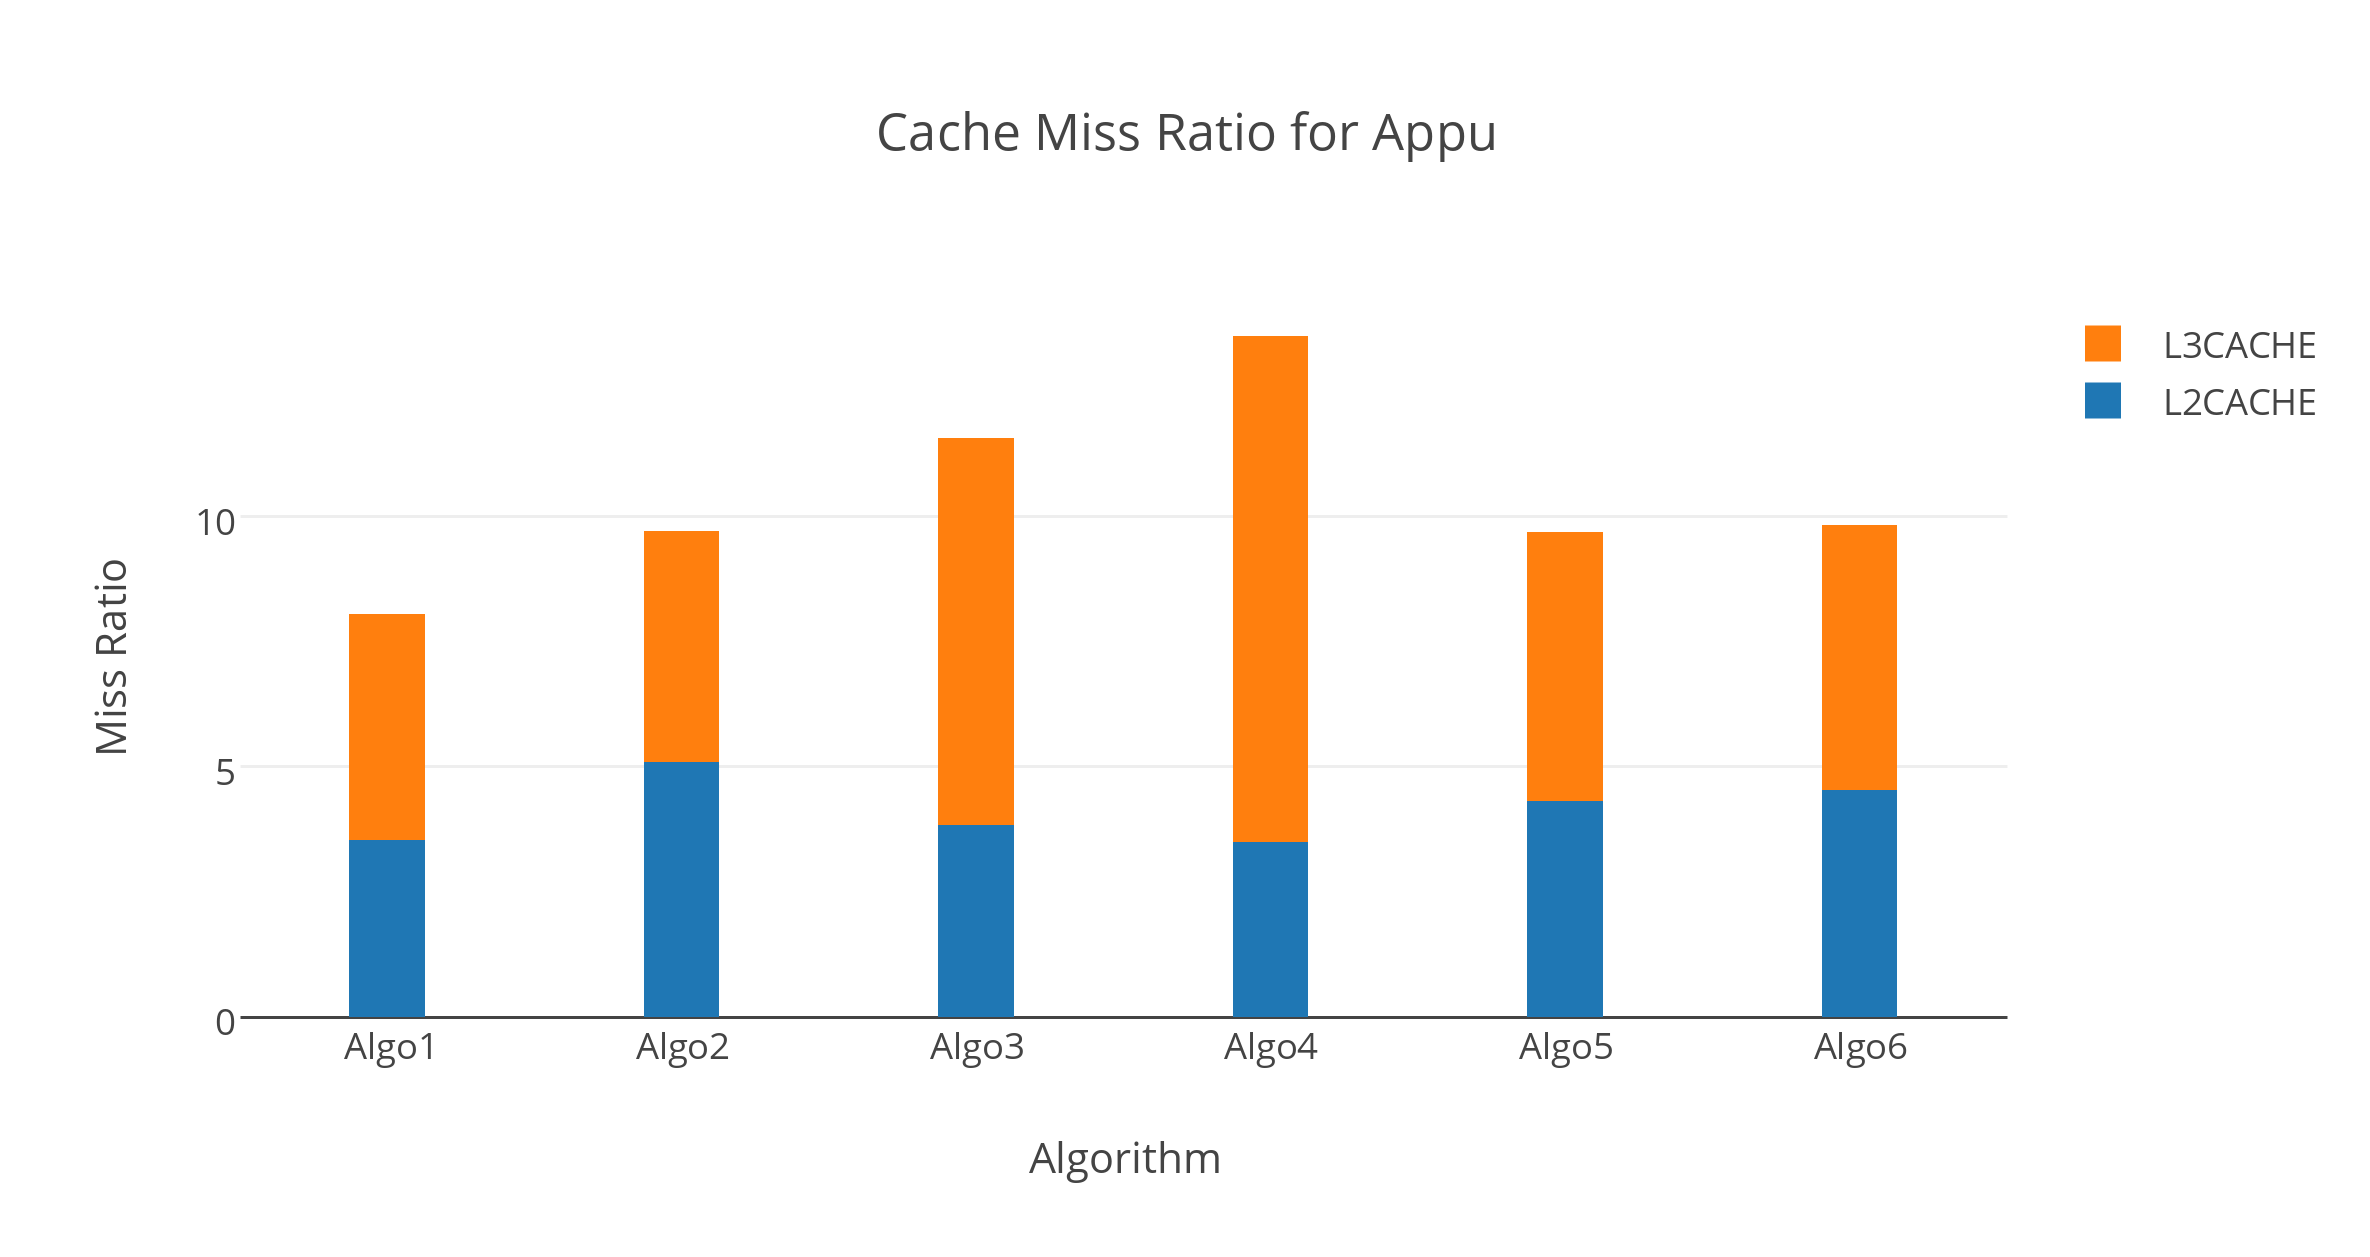
\includegraphics[width=0.5\textwidth]{figures/CacheMissRatioforAppu.eps}
    \caption{Cache-miss ratio for Appu}
    \label{fig:Appu-Cache Miss}
\end{figure}

\begin{figure}[t]
    \centering
    \includegraphics[width=0.5\textwidth]{figures/CacheMissRatioforDelaunay.eps}
    \caption{Cache-miss ratio for Delaunay}
    \label{fig:Delaunay-Cache Miss}
\end{figure}

\begin{figure}[t]
    \centering
    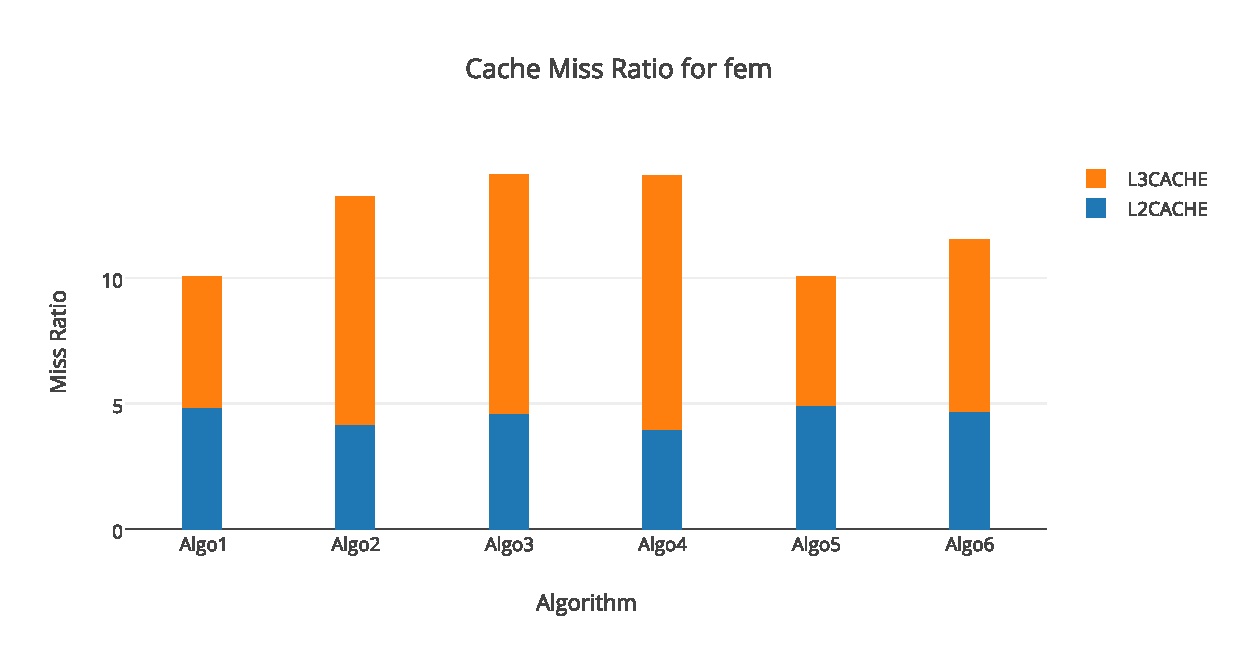
\includegraphics[width=0.5\textwidth]{figures/CacheMissRatioforFem.eps}
    \caption{Cache-miss ratio for Fem}
    \label{fig:Fem-Cache Miss}
\end{figure}

\begin{figure}[t]
    \centering
    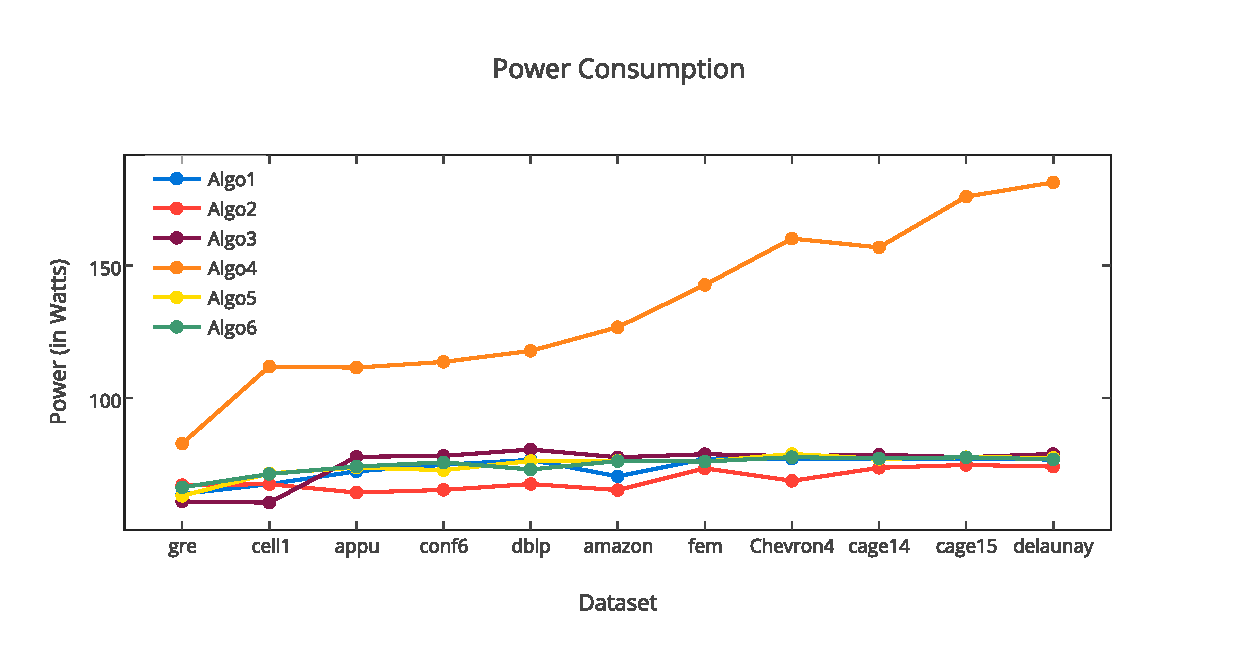
\includegraphics[width=0.5\textwidth]{figures/PowerConsumption.eps}
    \caption{Power Consumption}
    \label{fig:Power Consumption}
\end{figure}


\begin{figure}[t]
    \centering
    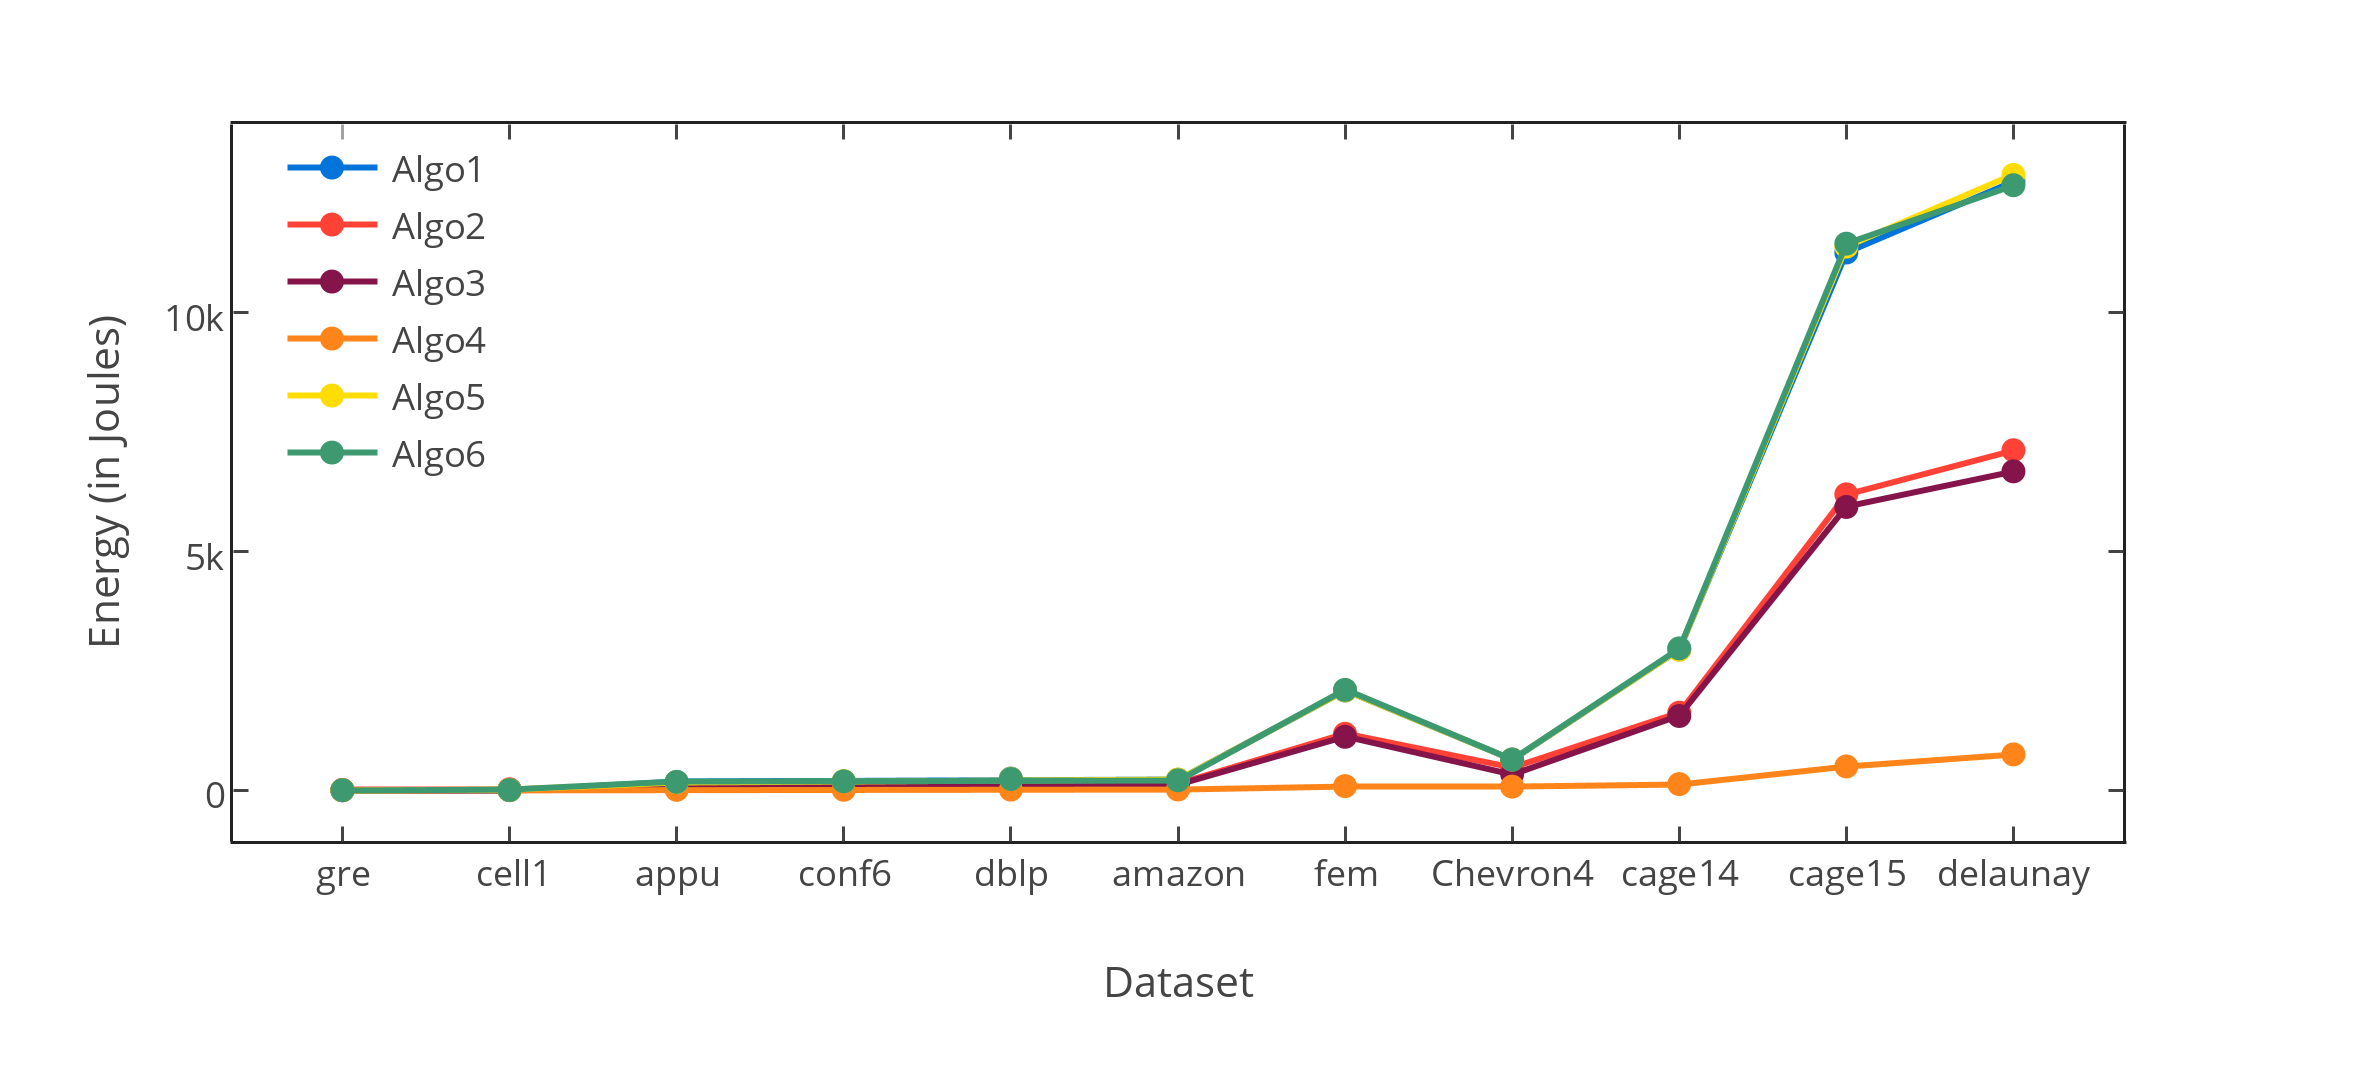
\includegraphics[width=0.5\textwidth]{figures/EnergyConsumption.eps}
    \caption{Energy Consumption}
    \label{fig:Energy Consumption}
\end{figure}


\begin{figure}[t]
    \centering
    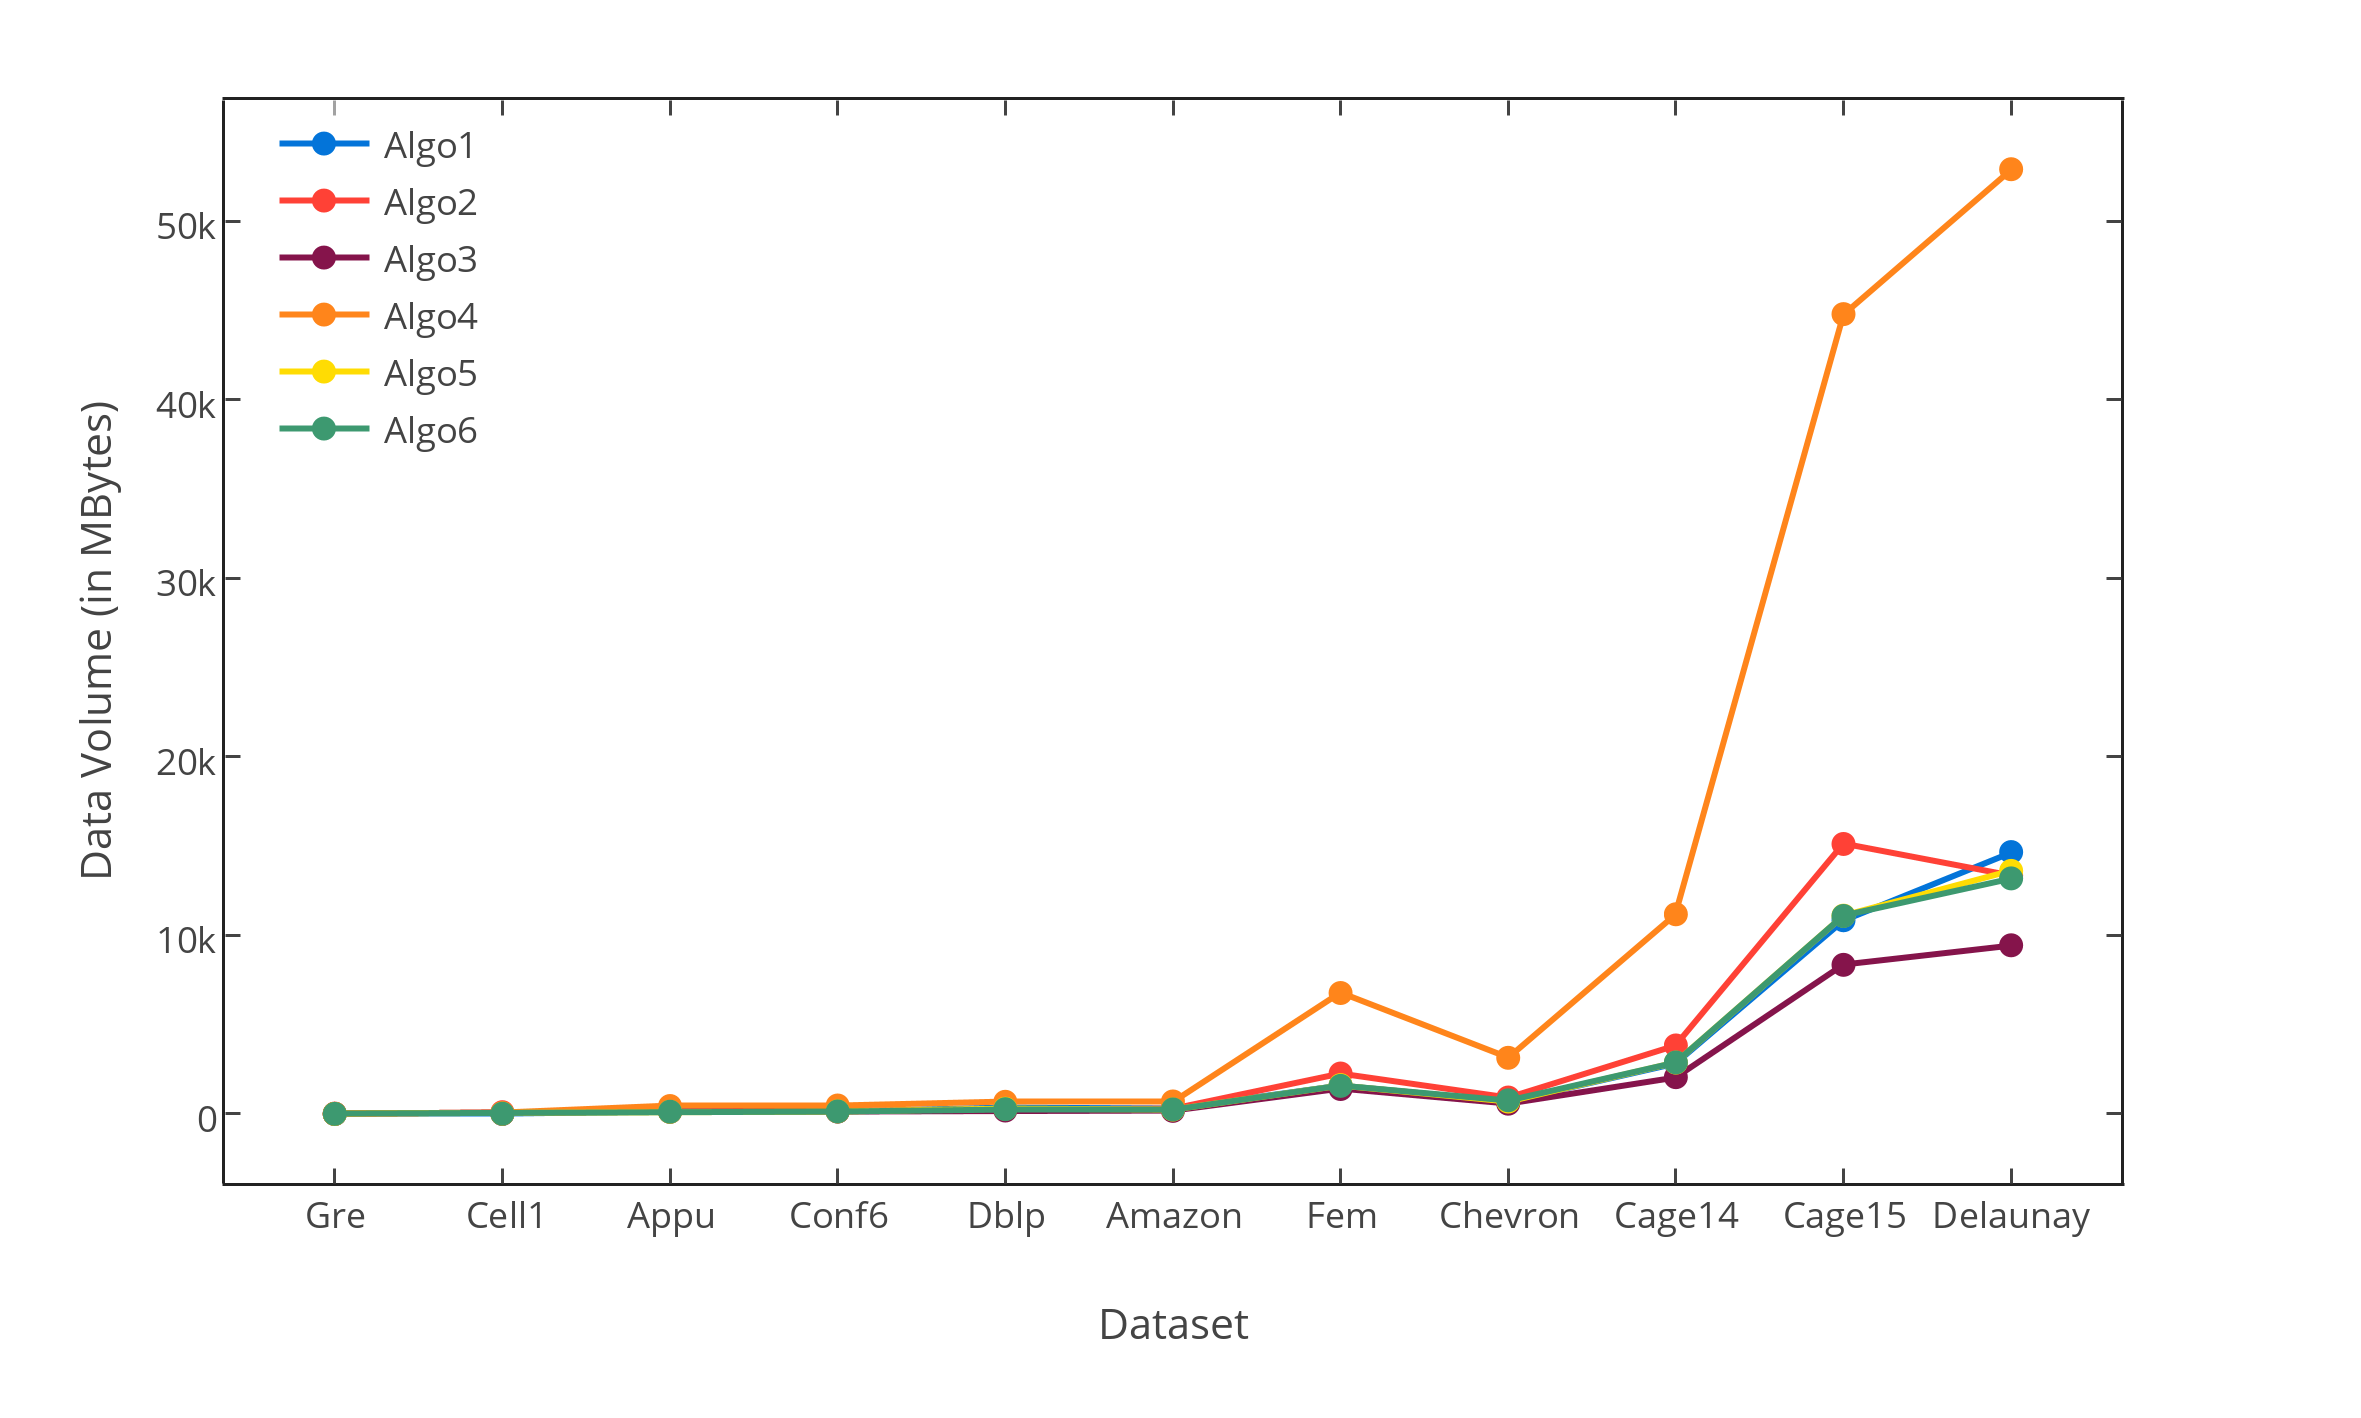
\includegraphics[width=0.5\textwidth]{figures/MEM-DataVolumeReadings.eps}
    \caption{MEM Consumption}
    \label{fig:MEM Consumption}
\end{figure}

\begin{figure}[t]
    \centering
    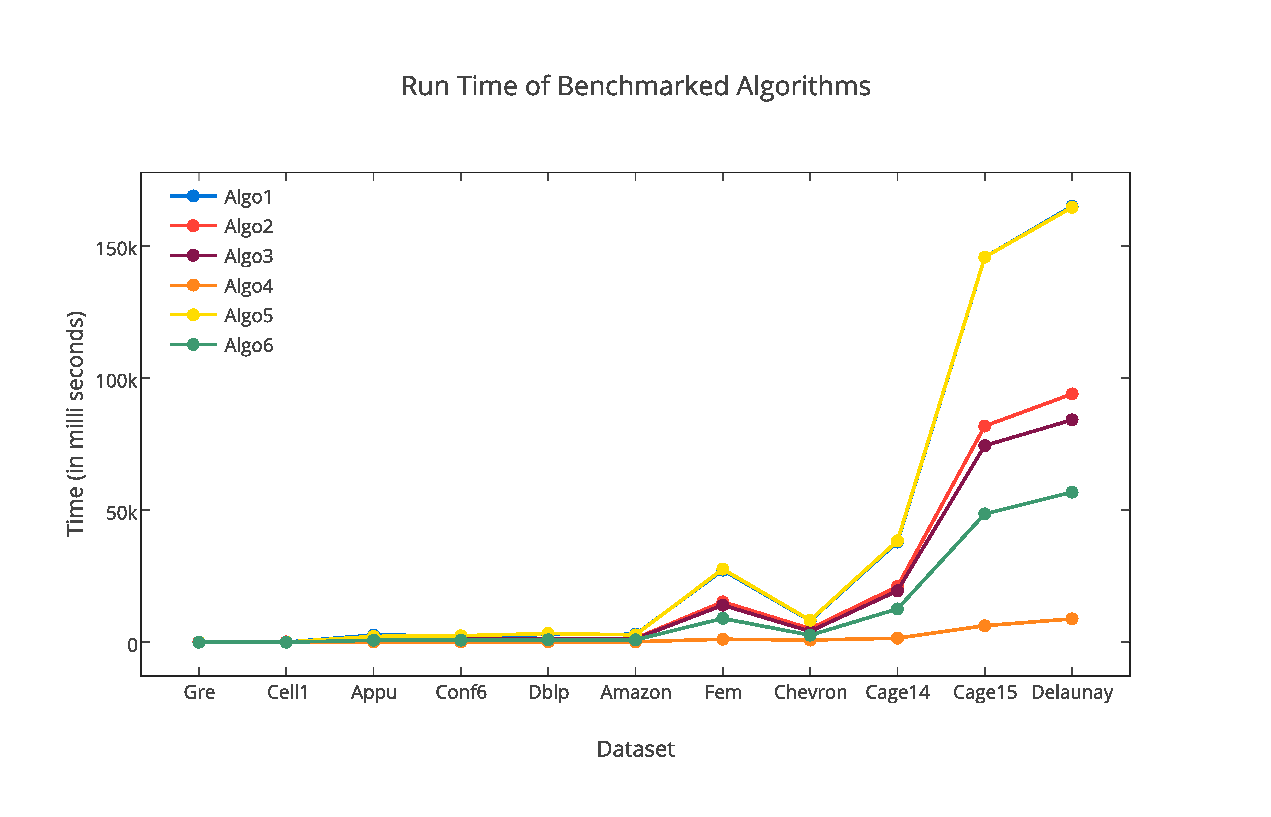
\includegraphics[width=0.5\textwidth]{figures/RunTimeofBenchmarkedAlgorithms.eps}
    \caption{Run Time (in ms)}
    \label{fig:Run Time}
\end{figure}

\paragraph{MEM performance}
From Table~\ref{tab:Table3} we can see that Algo3 performs the best
for most of the times.

\paragraph{L2CACHE performance}
From Table~\ref{tab:Table6} we can see that Algo4 performs best for
most of the times.

\paragraph{L3CACHE performance}
From Table~\ref{tab:Table6} we can see that Algo1 performs best for
most of the times.

\paragraph{Energy efficiency}
From Table~\ref{tab:Table5} we can see that Algo4 performs best for
most of the times. It reduces the work by avoiding an the re-visit of
already explored nodes, so overall energy consumption is minimal.

\paragraph{POWER efficiency}
Normally a machine consumes a constant amount of power if operated
with default parameters. But from Table~\ref{tab:Table5} we can see
that \emph{Algo4} takes the highest amount of power. This behavior can
be attributed to its inherent design to exploit max amount of
parallelism from the hardware.  To verify this we used the same
CPU and thread parameters for each algorithm, still Algo4 consumes max
power.

























%%%%%%%%%%%%%%%%%%%%%%%%%%%%%%%%%%%%%%%%%%%%%%%%%%%%%%%%%%%%%%%%%%%%%%%%%%%%%%%
% Table(s) for results of current experiments
%%%%%%%%%%%%%%%%%%%%%%%%%%%%%%%%%%%%%%%%%%%%%%%%%%%%%%%%%%%%%%%%%%%%%%%%%%%%%%

\begin{table*}[th]
\small
\centering
%\begin{tabularx}{\linewidth}{|c|c|c|c|c|c|c|X|}

\begin{tabular}{ c|c|c|c|c|c|c|c|c| }
  \cline{2-9}
  & 
  \multicolumn{2}{c}{\textbf{$u_{1}$}} &
  \multicolumn{2}{|c}{\textbf{$u_{2}$}} &
  \multicolumn{2}{|c}{\textbf{$u_{3}$}} &
  \multicolumn{2}{|c|}{\textbf{root}}  \\
  \cline{2-9}
  \multicolumn{1}{c|}{} &
  with & without & with & without & with & without & with & without\\
  \multicolumn{1}{c|}{} &
  change & changes & changes & changes & changes & changes & changes &
  changes\\
  \hline
  \multicolumn{1}{|c|}{\textbf{create file}}
  & Y & Y & N & Y & N & Y & N & Y \\
  \hline
  \multicolumn{1}{|c|}{\textbf{create dir}}
  & Y & Y & N & Y & N & Y & N & Y \\
  \hline
  \multicolumn{1}{|c|}{\textbf{remove file}}
  & Y & Y & N & Y & N & Y & N & Y \\
  \hline
  \multicolumn{1}{|c|}{\textbf{remove dir}}
  & Y & Y & N & Y & N & Y & N & Y \\
  \hline
  \multicolumn{1}{|c|}{\textbf{create symlink}}
  & Y & Y & N & Y & N & Y & N & Y \\
  \hline
  \multicolumn{1}{|c|}{\textbf{read symlink}}
  & Y & Y & N & Y & N & Y & N & Y \\
  \hline
  \multicolumn{1}{|c|}{\textbf{write symlink}}
  & Y & Y & N & Y & N & Y & N & Y \\
  \hline
  \multicolumn{1}{|c|}{\textbf{create hardlink}}
  & Y & Y & N & Y & N & Y & N & Y \\
  \hline
  \multicolumn{1}{|c|}{\textbf{write hardlink}}
  & Y & Y & N & Y & N & Y & N & Y \\
  \hline
  \multicolumn{1}{|c|}{\textbf{stat}}
  & Y & Y & N & Y & N & Y & N & Y \\
  \hline
  \multicolumn{1}{|c|}{\textbf{change dir}}
  & Y & Y & N & Y & N & Y & N & Y \\
  \hline
  \multicolumn{1}{|c|}{\textbf{read file}}
  & Y & Y & N & Y & N & Y & N & Y \\
  \hline
  \multicolumn{1}{|c|}{\textbf{write file}}
  & Y & Y & N & Y & N & Y & N & Y \\
  \hline
  \multicolumn{1}{|c|}{\textbf{create tar}}
  & Y & Y & N & Y & N & Y & N & Y \\
  \hline
  \multicolumn{1}{|c|}{\textbf{untar}}
  & Y & Y & N & Y & N & Y & N & Y \\
  \hline
  \multicolumn{1}{|c|}{\textbf{make}}
  & Y & Y & N & Y & N & Y & N & Y \\
  \hline
  \multicolumn{1}{|c|}{\textbf{rename}}
  & Y & Y & N & Y & N & Y & N & Y \\
  \hline
\end{tabular}

%\end{tabularx}
\caption{\capfont Results of different file system operations for
different users, with and without the changes.}
\label{tab:results}
\end{table*}

%%%%%%%%%%%%%%%%%%%%%%%%%%%%%%%%%%%%%%%%%%%%%%%%%%%%%%%%%%%%%%%%%%%%%%%%%%%%%%
%% For Emacs:
% Local variables:
% fill-column: 70
% End:
%%%%%%%%%%%%%%%%%%%%%%%%%%%%%%%%%%%%%%%%%%%%%%%%%%%%%%%%%%%%%%%%%%%%%%%%%%%%%%
%% For Vim:
% vim:textwidth=70
%%%%%%%%%%%%%%%%%%%%%%%%%%%%%%%%%%%%%%%%%%%%%%%%%%%%%%%%%%%%%%%%%%%%%%%%%%%%%%
% LocalWords:  PEAFS PEAIO Lustre SBU HMC config

%%%%%%%%%%%%%%%%%%%%%%%%%%%%%%%%%%%%%%%%%%%%%%%%%%%%%%%%%%%%%%%%%%%%%%%%%%%%%%%
% Table(s) for results of current experiments
%%%%%%%%%%%%%%%%%%%%%%%%%%%%%%%%%%%%%%%%%%%%%%%%%%%%%%%%%%%%%%%%%%%%%%%%%%%%%%

\begin{table*}[th]
\small
\centering
%\begin{tabularx}{\linewidth}{|c|c|c|c|c|c|c|X|}

\begin{tabular}{ c|c|c|c|c|c|c| }
  \cline{2-7}
  & 
  \multicolumn{2}{c}{\textbf{root}} &
  \multicolumn{2}{|c}{\textbf{user1}} &
  \multicolumn{2}{|c|}{\textbf{root\_notallowed}}\\ 
  \cline{2-7}
  \multicolumn{1}{c|}{} &
  with & without & with & without & with & without\\
  \multicolumn{1}{c|}{} &
  changes & changes & changes & changes & changes & changes\\
  \hline
  \multicolumn{1}{|c|}{\textbf{xfstests}}
  & 56(68) & 56(68) & 32(68) & 32(68) & 0(68) & - \\
  \hline
  \multicolumn{1}{|c|}{\textbf{eCryptfs-tests}}
  & 25(25) & 25(25) & 22(25) & 22(25) & 0(25) & - \\
  \hline
\end{tabular}

%\end{tabularx}
\caption{\capfont Number of passed tests and total tests for
\emph{XFSTEST} and \emph{eCryptfs-tests} for different users, with and
without the changes.}
\label{tab:results-xfs}
\end{table*}

%%%%%%%%%%%%%%%%%%%%%%%%%%%%%%%%%%%%%%%%%%%%%%%%%%%%%%%%%%%%%%%%%%%%%%%%%%%%%%
%% For Emacs:
% Local variables:
% fill-column: 70
% End:
%%%%%%%%%%%%%%%%%%%%%%%%%%%%%%%%%%%%%%%%%%%%%%%%%%%%%%%%%%%%%%%%%%%%%%%%%%%%%%
%% For Vim:
% vim:textwidth=70
%%%%%%%%%%%%%%%%%%%%%%%%%%%%%%%%%%%%%%%%%%%%%%%%%%%%%%%%%%%%%%%%%%%%%%%%%%%%%%
% LocalWords:  PEAFS PEAIO Lustre SBU HMC config

%
%\paragraph{Evaluation Goals}
%We aimed to provide a correct working solution for eCryptfs with minimal
%performance overheads.
%
%\begin{itemize}
%\item
%\textbf{Correctness}\\
%Only the users that are allowed to access, should be able to access
%the file contents.  Other users should get a permission denied error
%irrespective of their privilege level.
%
%The user who is assigned the administrative role should be able to add
%or revoke permissions to other users in the system.
%
%Users without administrative privilege should not be able to change
%file access policy or gain illegal access.
%\item
%\textbf{Performance}\\ Performance of underlying file system should
%not suffer a penalty due to this extra security enforcement in
%eCryptfs.
%
%We keep the policy management separate from data path, so there is no
%overhead from management tasks on system performance.
%\item
%\textbf{Regression testing}\\ This change should not break any
%existing functionality in eCryptfs as well as the underlying file
%system.
%
%We have tested our changes with basic file operations like create
%file, directory, symlink, delete, rename, untar, kernel compilation.
%We also have run more comprehensive tests such as
%\emph{XFSTESTS}~\cite{xfstests} and eCryptfs-utils test scripts.
%\end{itemize}
%
%\paragraph{Evaluation Plan}
%We have run a set of testing tools along with our manually written
%tests.  The tools are \emph{XFSTESTS} and test scripts provided in
%eCriptfs-utils.  We have run these tools on both modified and
%unmodified eCryptfs kernel for different users with different
%privilege level.  We have tried to run the maximum number of tests
%from these tools, in case of a test failure we rerun it in isolation and
%identify the root cause of failure.  Test cases from these tools are
%sufficient, as they test for the functionality and regression of the file
%system.
%
%\paragraph{Experimental Setup}
%We have used a virtual machine with two Intel\textregistered
%Xeon\texttrademark dual-core 2.40GHz CPUs, and 8GB RAM.  The machine
%ran \mbox{Ubuntu} 14.04.1 with a vanilla 3.19.5 Linux Kernel.  We
%chose \mbox{Ubuntu} because it is freely available and the package
%eCryptfs-utils is installed by default.  For our experiments, we have
%4 users $u_1$, $u_2$, $u_3$ and a root user.  Only user $u_1$ is
%authorized to access encrypted files.  User $u_2$ is placed in sudoer
%list, $u_3$ is a normal user.  All users have intention to access the
%encrypted data, so we have 3 type of attackers and one authorized
%user.
%
%
%\begin{figure}[t]
%    \centering
%    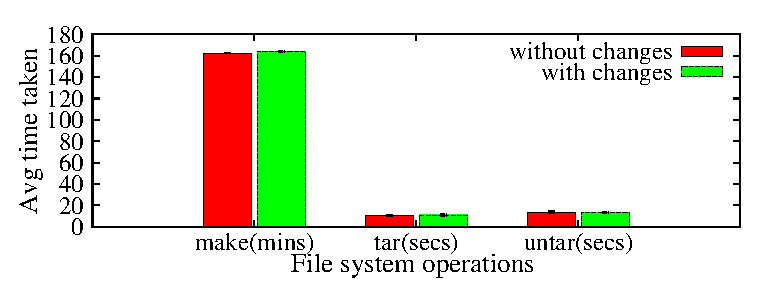
\includegraphics[width=0.5\textwidth]{figures/perf-results.eps}
%    \caption{eCryptfs performance comparison with and without our
%    changes for make, tar, untar operations.}
%    \label{fig:perf-results}
%\end{figure}
%
%
%\paragraph{Results}
%We ran basic file system operation for all four users mentioned above
%on the setup described.  We made changes to Linux Kernel 3.19.5.
%Table~\ref{tab:results} describes the results for all the file systems
%operations we ran.  Column 1 describes the file system operation.
%Column 2,3,4 shows results for users $u_1$, $u_2$, $u_3$ and root user
%respectively with and without our changes in Linux kernel.  \textbf{Y}
%indicates that the  operation ran successfully.  \textbf{N} indicates
%that the user was denied to run the corresponding commands inside the
%eCryptfs mount point.  We also ran some performance tests, such as
%make a Linux Kernel, tar/untar the source tree of Linux Kernel.
%Figure~\ref{fig:perf-results} shows that there is no significant
%performance overhead due to our changes.  The overhead for make workload
%is \emph{1.17\%} and for tar/untar is \emph{1.66\%}.
%
%We ran \emph{XFSTESTS} test-suite on Linux-3.19.5 vanilla kernel for
%\emph{eCryptfs} file system.  We used \emph{FSL} git repository of
%\emph{XFSTESTS} for our tests.  We modified the test-suite to support
%\emph{eCryptfs} file system.  These tests can be categorized in two
%categories, 1, without changes and 2, with changes in eCryptfs kernel
%code.  For category 1 we ran the test-suite for root user and a
%non-root user.  For category 2 we ran the test-suite for an allowed
%non-root user, and root user.  Then we added the root user to allowed
%users list and ran the test-suite again.  We compared the test results
%for both categories for each corresponding user.  We find there is no
%difference in the results.  We see that for category 2, when root user
%was not allowed to access eCryptfs file system, all tests failed.
%
%We also found new interesting bugs with eCryptfs file system.
%\begin{itemize}
%\item 
%\textbf{noatime mount option:} If the eCryptfs file system is mounted
%with noatime mount option, the access times for any file should never
%change.  But we see that there is no difference between if file system
%is mounted with noatime option or not.  The access time for files
%changes in both the cases.
%
%\item
%\textbf{Direct IO:} eCryptfs does not support direct IO.  So all the
%tests for direct IO failed.
%\item
%\textbf{File access timestamp Epoch:} Create a file in eCryptfs
%directory with creation time before epoch.  Check the time of last
%access as seconds since Epoch, it should be a negative value.  Now
%flush the cache by remounting the file system.  Now if we check again
%for the time of last access as seconds since Epoch, it should still be
%negative, but that is not the case here.
%\end{itemize}
%
%All the \emph{XFSTESTS} that failed can be assigned to the issues
%mentioned above.
%
%We also ran the default eCryptfs-test script found in eCryptfs utils.
%These tests include various file systems tests, such as file read,
%write, concurrent access, inode races, symlinks, file truncate.  These
%tests also include tests for already identified bugs in eCryptfs.
%These tests ensures that we did not break anything that was working
%before our changes.  For both the categories, we did not find any
%difference in the results for all the tests.  As expected for any
%non-allowed user all the tests in the script failed.
%
%Table~\ref{tab:results-xfs} shows the number of tests that passed from
%total number of tests for both the test-suites for various users.  We
%examined the failed tests and identified why some of \emph{XFSTESTS}
%failed.  The numbers show that there was nothing broken due to our
%changes.  Since many tests requires root permissions as these are
%kernel level tests, the amount of tests that failed for non-root user
%were considerably higher than that of root user.
%
%IOCTL interface is restricted to admin user.  For our experiments we
%hard coded a UID \mbox{1234} as admin user in eCryptfs kernel.  We
%created a user with UID \mbox{1234} using adduser(1) utility.  At
%mount time only admin user is added to the list of allowed users.
%Root can mount the file system but cannot access the files within the
%mount point, as it is not part of allowed list.  At this point only
%admin user can perform file operation and user management activity.
%Once the admin added a user to the set of allowed users, that user can
%perform file operation.  Still user management operations like
%list\_users/allow\_user/revoke\_user is restricted to admin user.
%
%We tested IOCTL interface via multiple users like admin, user1, user2,
%root.  We observed that only admin user was able to successfully run
%the IOCTL commands, other users including root got permission denied
%error.  Since admin role is non-revocable, even the admin user cannot
%revoke itself.  Admin user cannot add any users to the allowed list
%once the list was full, too many users error is returned.  We verified
%that the file operation path was being properly affected by the
%changes done via IOCTL interface.
%
%%%%%%%%%%%%%%%%%%%%%%%%%%%%%%%%%%%%%%%%%%%%%%%%%%%%%%%%%%%%%%%%%%%%%%%%%%%%%%
%% For Emacs:
% Local variables:
% fill-column: 70
% End:
%%%%%%%%%%%%%%%%%%%%%%%%%%%%%%%%%%%%%%%%%%%%%%%%%%%%%%%%%%%%%%%%%%%%%%%%%%%%%%
%% For Vim:
% vim:textwidth=70
%%%%%%%%%%%%%%%%%%%%%%%%%%%%%%%%%%%%%%%%%%%%%%%%%%%%%%%%%%%%%%%%%%%%%%%%%%%%%%
% LocalWords:

%\section{Related Work}
\label{related}

%Related work section...
%
%Typical length: 0.5-2.0 papers, avg 1.0 (assuming a 12-14
%conf. paper).
%
%Background and Related Work can be similar.
%Most citations will be in this section.
%
%Describe past work and criticize it, fairly.  Use citations to
%JUSTIFY your criticism! Now you can fairly compare to YOUR work.
%
%Problem: don't put background/motivation material here (too
%late).
%
%Important: when it doubt, cite it! (to avoid not citing a
%reviewer's own papers, or papers they know or "think" are
%related).
%
%If conf. allows unlimited citations, do so.
%
%Organize past work: should it be importance order?
%chronological? categorical?

File based encryption are popular and have been deployed widely.  Matt
Blaze designed Cryptographic File System (CFS) pushes encryption
services into the file system itself~\cite{cfs}.  CFS supports secure
storage at the system level through a standard Unix file system
interface to encrypted files.  Users associate a cryptographic key
with the directories they wish to protect.  Files in these directories
(as well as their pathname components) are transparently encrypted and
decrypted with the specified key without further user intervention;
plain text is never stored on a disk or sent to a remote file server.
CFS can use any available file system for its underlying storage
without modification, including remote file servers such as NFS.
System management functions, such as file backup, work in a normal
manner and without knowledge of the key.

EncFS is a user-space stackable cryptographic file-system similar to
eCryptfs, and aims to secure data with the minimum
hassle~\cite{encfs}.  It uses FUSE to mount an encrypted directory
onto another directory specified by the user.  It does not use a
loopback system like some other comparable systems such as TrueCrypt
and dm-crypt.

Existing cryptographic file systems for Unix do not take into account
that sensitive data must often be shared with other users, but still
kept secret.  By design, the only one who has access to the secret
data is the person who encrypted it and therefore knows the encryption
key or password.  This paper presents a kernel driver for a new
encrypted file system, called Fairly Secure File System (FSFS), which
provides mechanisms for user management and access control for
encrypted files~\cite{fsfs}.  The driver has been specifically
designed with multi user systems in mind.  FSFS also tries to prevent
unintentional transfer of sensitive data to unencrypted file systems,
where it would be stored in plain text.


%%%%%%%%%%%%%%%%%%%%%%%%%%%%%%%%%%%%%%%%%%%%%%%%%%%%%%%%%%%%%%%%%%%%%%%%%%%%%%
%% For Emacs:
% Local variables:
% fill-column: 70
% End:
%%%%%%%%%%%%%%%%%%%%%%%%%%%%%%%%%%%%%%%%%%%%%%%%%%%%%%%%%%%%%%%%%%%%%%%%%%%%%%
%% For Vim:
% vim:textwidth=70
%%%%%%%%%%%%%%%%%%%%%%%%%%%%%%%%%%%%%%%%%%%%%%%%%%%%%%%%%%%%%%%%%%%%%%%%%%%%%%
% LocalWords:  SMR HDDs drive's SMRs

\section{Conclusions}
\label{conc}

%Conclusion text...
%
%Length: 0.25-0.5 pages max (1-2 pgfs)
%
%Summary of key contributions (should match your design goals).
%Not summary of whole paper.  Any novel contributions mentioned.
%Summarize good eval results.
%
%Key: give reader the "take home" message.

We have presented a comprehensive benchmarking study of BFS algorithms
and reported their performance in terms of ENERGY, MEMORY and CACHE
performance.  Our study found that Algorithm 4 ~\cite{LIGRA-BFS} is the most
energy efficient.  This can be attributed to its extremely good running time
and L2CACHE performance.
\newline
Also, we observe that Algorithm 1 is L3CACHE efficient, and Algorithm 3 is
MEMORY efficient.  This indicates that no algorithm performs best for
all the parameters, they optimize one parameter at the expense of another.

%which can be attributed to its \emph{hybrid} implementation.  We do
%observe a clear winner in terms of execution time,  Algo4 is the most
%run-time efficient which also makes it energy efficient.

\paragraph{Future Work}
We plan to extend our project to some more Scale-Free datasets.  Now
that we have analysed BFS algorithms for energy related parameters, to
widen our understanding we would like to benchmark other graph
algorithms like \emph{Connected Components} or \emph{Minimum Spanning
Tree}. We also plan to run the experiments on \emph{scale-free} graph
datasets.
\newline
With our understanding of how these parameters behave and their affect
on performance, in future we plan to extend some existing BFS
algorithm to achieve energy efficiency.

%Future work text...
%
%Typical length: 0.25-0.33 pages max
%
%Don't write too much:
%- the more you write, the more work appears "premature"
%- takes up important space (small impact on acceptance)
%
%Often folded as subsection of conclusions.
%
%Describe most important 1-3 "novel/research" future work ideas.
%
%Avoid "short term" future goals.  Focus on long-term goals, well
%beyond the scope of THIS paper.  Avoid stuff that might be
%considered as should have been part of this work.
%
%Give reader some ideas of HOW you plan to go about investigating
%future ideas.
%

%%%%%%%%%%%%%%%%%%%%%%%%%%%%%%%%%%%%%%%%%%%%%%%%%%%%%%%%%%%%%%%%%%%%%%%%%%%%%%
%% For Emacs:
% Local variables:
% fill-column: 70
% End:
%%%%%%%%%%%%%%%%%%%%%%%%%%%%%%%%%%%%%%%%%%%%%%%%%%%%%%%%%%%%%%%%%%%%%%%%%%%%%%
%% For Vim:
% vim:textwidth=70
%%%%%%%%%%%%%%%%%%%%%%%%%%%%%%%%%%%%%%%%%%%%%%%%%%%%%%%%%%%%%%%%%%%%%%%%%%%%%%
% LocalWords:

\paragraph{Acknowledgments}
\label{ack}

%1 pgf max.
%
%Optional if you have space.  Cannot ack in anonymous
%submissions.
%
%List anyone who helped ideas, review drafts, but isn't a
%co-author.
%
%List any funding agency that supported the work (some agencies
%require this).
%
%Example:
%
%We thank the EMC/Data Domain performance team for their help.  We also
%thank Windsor Hsu, our shepherd Jiri Schindler and our anonymous
%reviewers for their helpful feedback.  This work was supported in part
%by NSF award CCF-0937854.

We thank Professor Erez Zadok for guidance and rigorous design reviews.
We also thank Ming Chen for helping with the \emph{XFSTESTS}.

%%%%%%%%%%%%%%%%%%%%%%%%%%%%%%%%%%%%%%%%%%%%%%%%%%%%%%%%%%%%%%%%%%%%%%%%%%%%%%
%% For Emacs:
% Local variables:
% fill-column: 70
% End:
%%%%%%%%%%%%%%%%%%%%%%%%%%%%%%%%%%%%%%%%%%%%%%%%%%%%%%%%%%%%%%%%%%%%%%%%%%%%%%
%% For Vim:
% vim:textwidth=70
%%%%%%%%%%%%%%%%%%%%%%%%%%%%%%%%%%%%%%%%%%%%%%%%%%%%%%%%%%%%%%%%%%%%%%%%%%%%%%
% LocalWords:  SMR HDDs drive's SMRs

%\clearpage

%\appendix
%\section{General Purpose Notes}

\subsection{Notes About Picking a Project}

Put every possible related citation you can! (esp. if conf.
doesn't count citations towards page size).

Literature survey:
- CiteSeer

- Google Scholar

- libraries

1. find a few relates paper

2. skim papers to find relevance

3. search for add'l related papers in Biblio.

4. reverse citation: use srch engines, to find
   newer papers that cite the paper you like.

5. "stop" when reach transitive closure

- then go off and read it; summarize papers

- think about "how can I improve" and "what was so
  good about that paper".

- check future work for project ideas.

- go to talks \& conferences

Pick an idea:

- novelty vs. incremental (how big of an increment?)

- idea vs. practical implications
  (implemented? released? in use as OSS or commercial?)

- where to submit? good fit and match for quality.

- look at schedule of conferences: due dates \& result dates.
i.e., what's the due dates, when do you hear an accept/reject
notice by; if the paper is rejected, where/when can you submit
it to next?

\subsection{Different Types of Technical Papers}

Computer systems field:

- operating systems, networking, security

- programming, virtualization, storage

- architecture, databases, etc.

- NOT: theory

1. conference paper: mature, completed work. [length 6-14 pages]

2. workshop paper: short, work-in-progress report [4-6 pp]

- special workshop type: a "position" paper, often called "Hot-???"

3. journal article: expanded version of a conference/workshop
   paper.  No page limit.  Common to follow up a workshop and even
   a conf. paper with an exapnded journal version. Journals often
   ask for at least 25\% more "new" material.

Conf./workshop/journals are "refereed" publications, meaning that
your peers get to review the document and accept/reject it, and
return comments to you.  Non-refereed pubs are usually called
"technical reports": anyone can publish a TR on their own.

Workshop and conf. papers get presented in person: usually lead
author would give the talk.  Journals are not presented.

In this class, you will submit a "position" paper (your design
document, 2 pp); by end of term, you'll submit a longer conf. like'
paper (6+ pp).

Conf./workshop papers review cycle: 1-4 months

- journals: no time limit; often; no deadline often 6+ months.

Conf./workshop papers get an accept/reject notice:

- rate: a conditional accept pending "shepherd's aproval"

Journals: phases of aproval:

- reject: "go away"

- major revision: a reject; ask to make major changes and resubmit.

- minor revision: a reject; ask to make minor changes and resubmit.

- conditional accept: very minor changes asked (usually prose,
  typos, English)

- accept: manuscript is accepted as is.

Publishing cycles, from moment of receiving an "accept notice":

- workshop/conf.: 2-3 months; present @ venue 2-3 months later.

- journal: 2-6 months

A manuscript is considered published on 1st day of workshop/conf.
or the first day of the month in which the journal is published.

%%%%%%%%%%%%%%%%%%%%%%%%%%%%%%%%%%%%%%%%%%%%%%%%%%%%%%%%%%%%%%%%%%%%%%%%%%%%%%
%% For Emacs:
% Local variables:
% fill-column: 70
% End:
%%%%%%%%%%%%%%%%%%%%%%%%%%%%%%%%%%%%%%%%%%%%%%%%%%%%%%%%%%%%%%%%%%%%%%%%%%%%%%
%% For Vim:
% vim:textwidth=70
%%%%%%%%%%%%%%%%%%%%%%%%%%%%%%%%%%%%%%%%%%%%%%%%%%%%%%%%%%%%%%%%%%%%%%%%%%%%%%
% LocalWords:  SMR HDDs drive's SMRs




\bibliographystyle{plain}
\bibliography{template/master,smr}
%{\footnotesize \bibliography{template/master}}

%\newpage

\end{document}

%%%%%%%%%%%%%%%%%%%%%%%%%%%%%%%%%%%%%%%%%%%%%%%%%%%%%%%%%%%%%%%%%%%%%%%%%%%%%%
%% For Emacs:
% Local variables:
% fill-column: 70
% End:
%%%%%%%%%%%%%%%%%%%%%%%%%%%%%%%%%%%%%%%%%%%%%%%%%%%%%%%%%%%%%%%%%%%%%%%%%%%%%%
%% For vim:
% vim:textwidth=70
%%%%%%%%%%%%%%%%%%%%%%%%%%%%%%%%%%%%%%%%%%%%%%%%%%%%%%%%%%%%%%%%%%%%%%%%%%%%%%
% LocalWords:

% LocalWords:  Ankur Agrawal Benixon Arul Dhas Hospodor Yangwook Kang Rekha UC
% LocalWords:  Pitchumani Sphurti Sortur USletter csrg smr
